\pdfminorversion=4
\documentclass[aspectratio=169]{beamer}

\mode<presentation>
{
  \usetheme{default}
  \usecolortheme{default}
  \usefonttheme{default}
  \setbeamertemplate{navigation symbols}{}
  \setbeamertemplate{caption}[numbered]
  \setbeamertemplate{footline}[frame number]  % or "page number"
  \setbeamercolor{frametitle}{fg=white}
  \setbeamercolor{footline}{fg=black}
} 

\usepackage[english]{babel}
\usepackage{inputenc}
\usepackage{tikz}
\usepackage{courier}
\usepackage{array}
\usepackage{bold-extra}
\usepackage{minted}
\usepackage[thicklines]{cancel}
\usepackage{fancyvrb}
\usepackage{setspace}

\xdefinecolor{dianablue}{rgb}{0.18,0.24,0.31}
\xdefinecolor{darkblue}{rgb}{0.1,0.1,0.7}
\xdefinecolor{darkgreen}{rgb}{0,0.5,0}
\xdefinecolor{darkgrey}{rgb}{0.35,0.35,0.35}
\xdefinecolor{darkorange}{rgb}{0.8,0.5,0}
\xdefinecolor{darkred}{rgb}{0.7,0,0}
\definecolor{darkgreen}{rgb}{0,0.6,0}
\definecolor{mauve}{rgb}{0.58,0,0.82}

\title[2022-09-28-future-trends-python]{Status of Analysis --- The Python Perspective}
\author{Jim Pivarski}
\institute{Princeton University -- IRIS-HEP}
\date{September 28, 2022}

\usetikzlibrary{shapes.callouts}

\begin{document}

\logo{\pgfputat{\pgfxy(0.11, 7.4)}{\pgfbox[right,base]{\tikz{\filldraw[fill=dianablue, draw=none] (0 cm, 0 cm) rectangle (50 cm, 1 cm);}\mbox{\hspace{-8 cm}
\includegraphics[height=1 cm]{princeton-logo-long.png}\hspace{0.1 cm}\raisebox{0.1 cm}{
\includegraphics[height=0.8 cm]{iris-hep-logo-long.png}}\hspace{0.1 cm}}}}}

\begin{frame}
  \titlepage
\end{frame}

\logo{\pgfputat{\pgfxy(0.11, 7.4)}{\pgfbox[right,base]{\tikz{\filldraw[fill=dianablue, draw=none] (0 cm, 0 cm) rectangle (50 cm, 1 cm);}\mbox{\hspace{-8 cm}
\includegraphics[height=1 cm]{princeton-logo.png}\hspace{0.1 cm}\raisebox{0.1 cm}{
\includegraphics[height=0.8 cm]{iris-hep-logo.png}}\hspace{0.1 cm}}}}}

% Uncomment these lines for an automatically generated outline.
%\begin{frame}{Outline}
%  \tableofcontents
%\end{frame}

% START START START START START START START START START START START START START

\begin{frame}{Something I want to address in this talk}
\vspace{0.1 cm}
\begin{center}
\only<1>{
\includegraphics[width=0.85\linewidth]{PLOTS/indico-future2022.png}}\only<2>{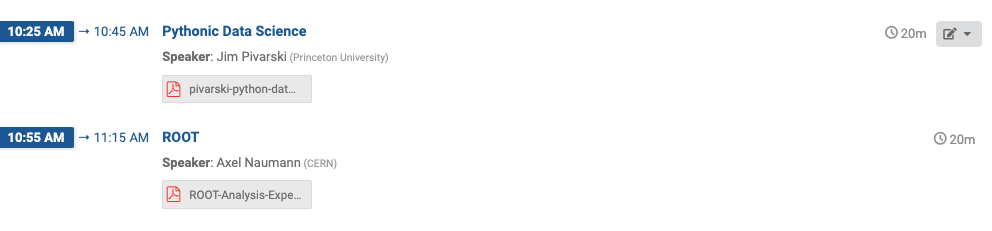
\includegraphics[width=0.85\linewidth]{PLOTS/indico-hllhc2021.png}}\only<3>{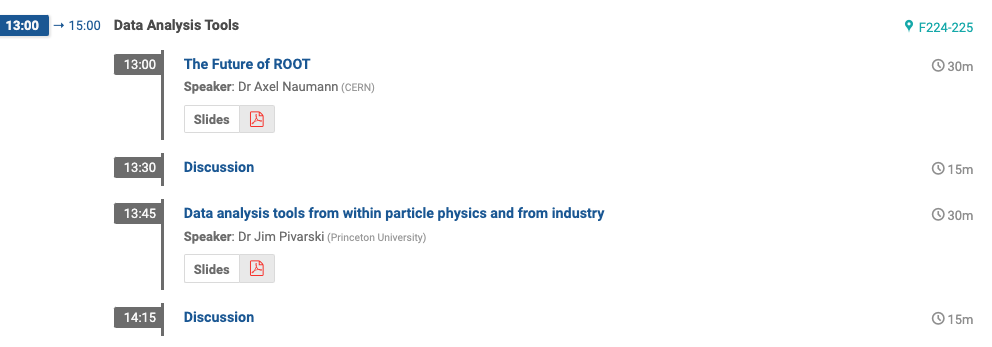
\includegraphics[width=0.85\linewidth]{PLOTS/indico-roundtable2018.png}}\only<4>{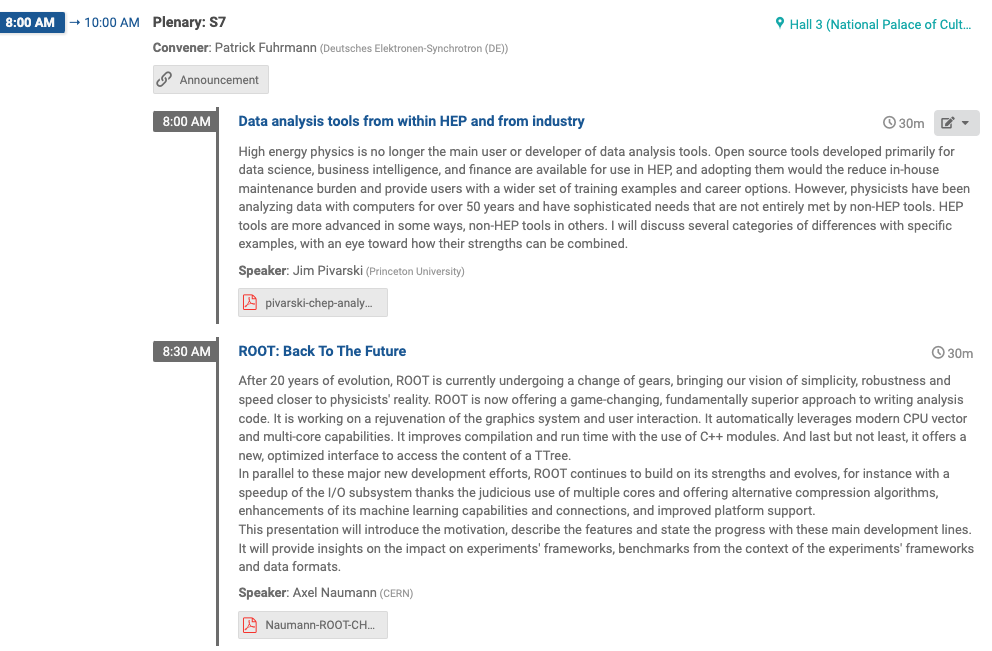
\includegraphics[width=0.85\linewidth]{PLOTS/indico-chep2018.png}}
\end{center}
\end{frame}

\begin{frame}{\mbox{ }}
\Large
It might be an efficient way to summarize all the analysis activities:
\begin{center}
Python $\bigcup$ ROOT.
\end{center}

\vspace{1 cm}
\uncover<2->{But sometimes people read into it an implicit ``versus.''}
\end{frame}

\begin{frame}{\mbox{ }}
\Large
\vspace{0.25 cm}
ROOT has had a Python interface since 2004.

\vspace{0.2 cm}
\begin{itemize}
\item<2-> PyROOT is old enough to vote!
\end{itemize}

\vspace{1.25 cm}
\begin{uncoverenv}<3->
Nor is the alternative strictly ``Python.''
\vspace{0.2 cm}
\begin{itemize}
\item<4-> I've also tried to characterize it as ``industry'' or ``data science.''
\end{itemize}
\end{uncoverenv}
\end{frame}

\begin{frame}{\mbox{ }}
\Large
What I'm trying to talk about here is a social trend, and using a programming language as a proxy for it.
\end{frame}

\begin{frame}{Analysis of 11\,635 GitHub repos created by 2\,172 CMS physicists}
\vspace{0.25 cm}

Software for the CMS experiment is on GitHub and only CMS physicists need to fork it. Using that, we can examine all of those physicists' non-fork, public repositories.

\vspace{0.2 cm}

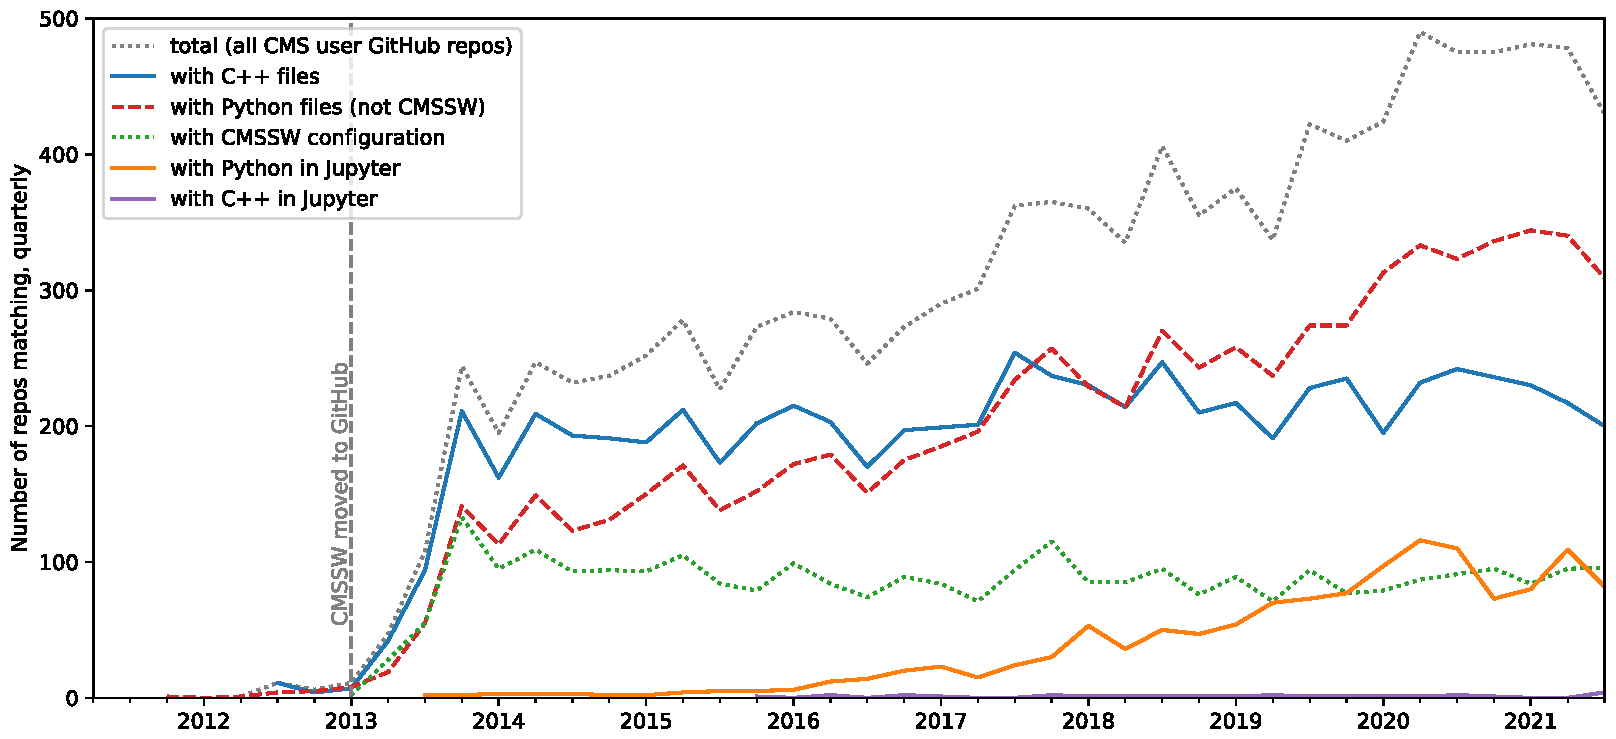
\includegraphics[width=\linewidth]{PLOTS/gihub-language-fullstudy.pdf}
\end{frame}

\begin{frame}{Analysis of 11\,635 GitHub repos created by 2\,172 CMS physicists}
\vspace{0.25 cm}

By regex searching for ``\mintinline{python}{import [A-Za-z_][A-Za-z_0-9]*}'' etc., we can count the number of physicist repositories that use different packages over time.

\vspace{0.2 cm}

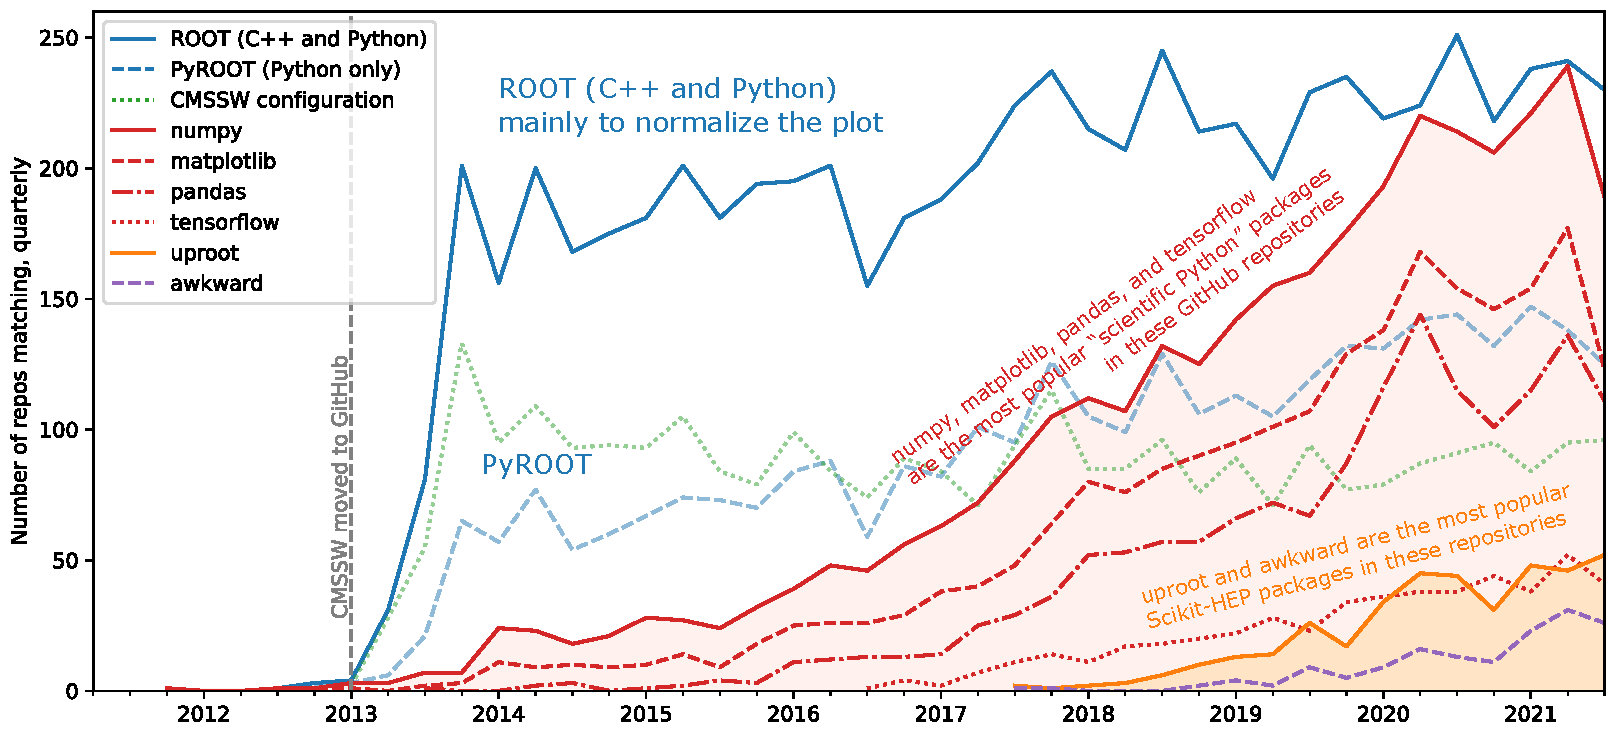
\includegraphics[width=\linewidth]{PLOTS/gihub-package-fullstudy.pdf}
\end{frame}

\begin{frame}[fragile]{\mbox{ }}
\Large
There is a rise in Python usage (including PyROOT).

\vspace{1.5 cm}
\begin{uncoverenv}<2->
But the biggest thing that happened in the past 5 years is

\begin{center}
\begin{minipage}{0.95\linewidth}
\begin{minted}{python}
import numpy, matplotlib, pandas, tensorflow
\end{minted}
\end{minipage}
\end{center}

\vspace{0.2 cm}
\begin{spacing}{1.0}
What we're seeing is the use of data analysis tools developed by scientists from other fields, the Big Data industry, quants, \dots
\end{spacing}
\end{uncoverenv}
\end{frame}

\begin{frame}{In fact, Python, the language, has been in HEP for a long time}
\vspace{0.25 cm}

Regex matches to all Computing in High Energy Physics (CHEP) titles and abstracts.

\vspace{-0.1 cm}
\begin{center}
\only<1>{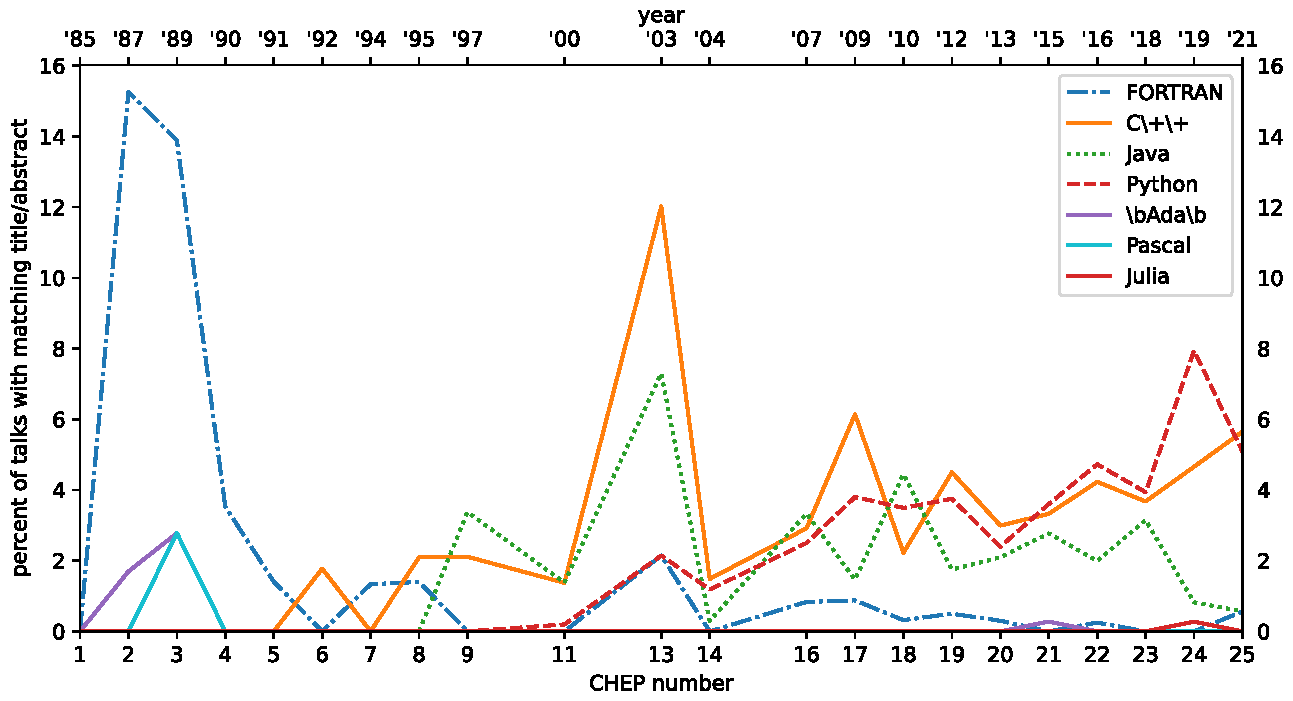
\includegraphics[width=0.95\linewidth]{PLOTS/chep-papers-language.pdf}}\only<2>{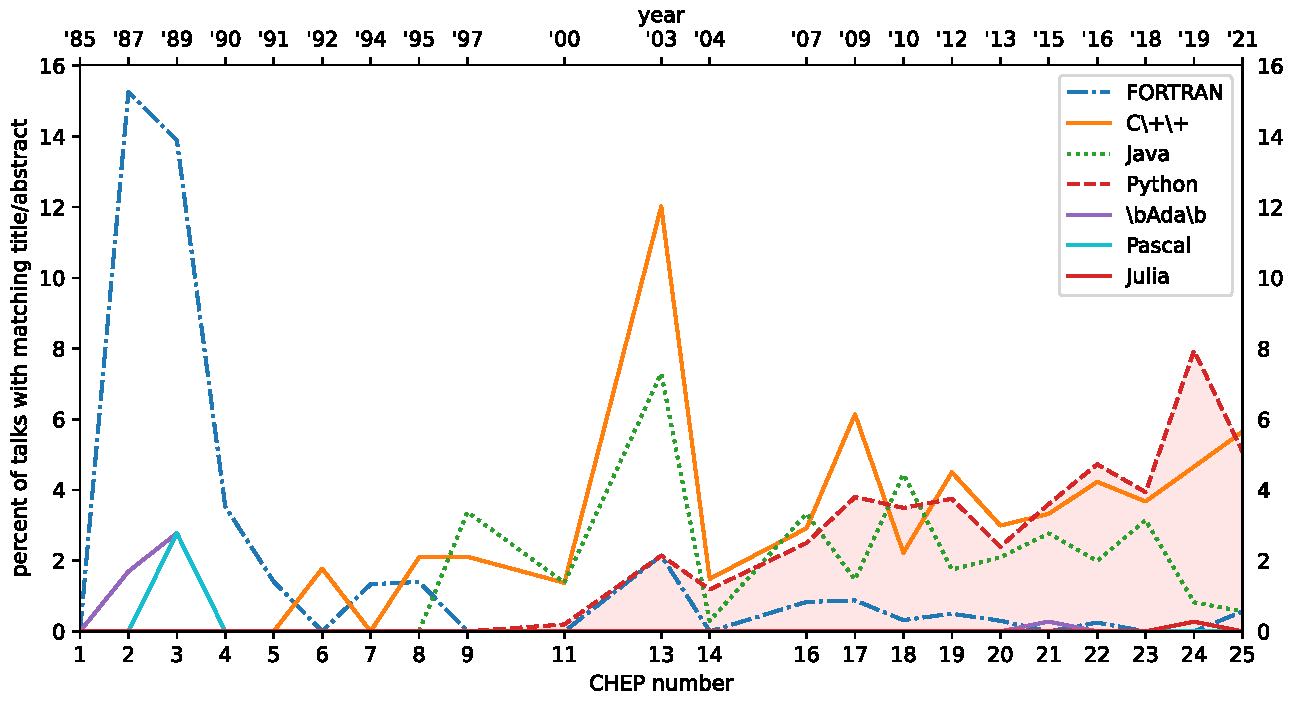
\includegraphics[width=0.95\linewidth]{PLOTS/chep-papers-language-shaded.pdf}}
\end{center}
\end{frame}

\begin{frame}{From Lucas Taylor's summary of data analysis track, CHEP 2001}
\vspace{0.25 cm}

\mbox{ } \hfill 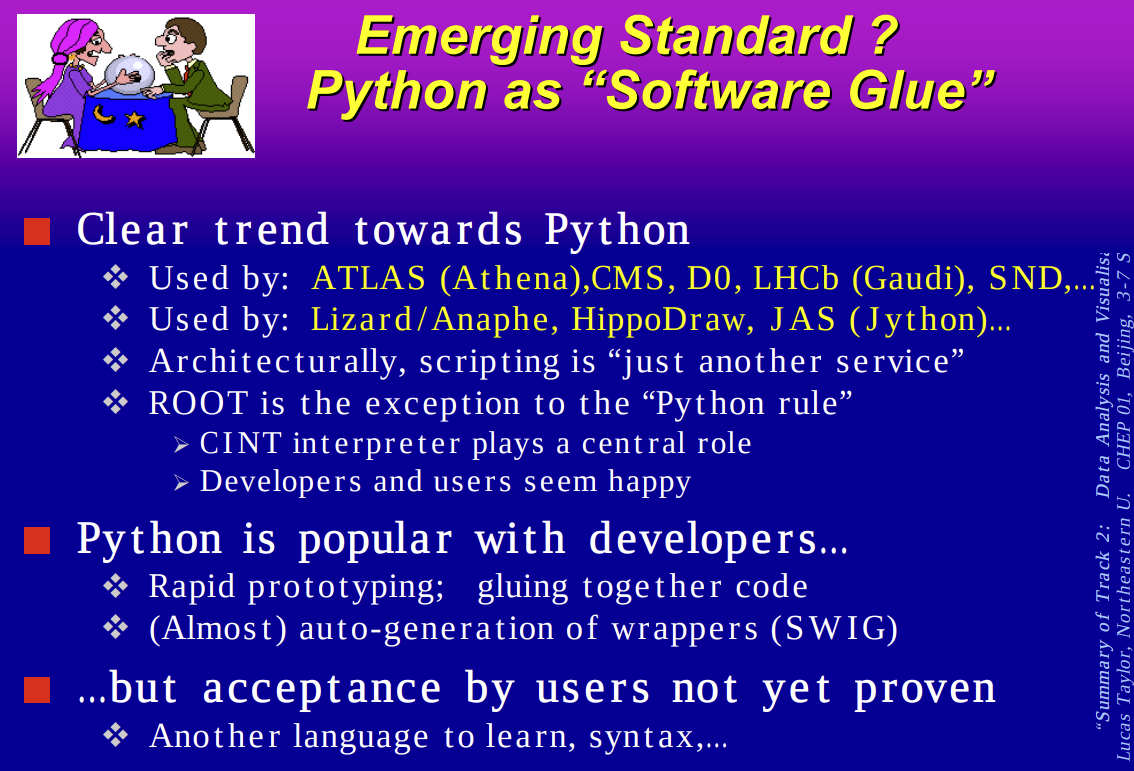
\includegraphics[width=0.82\linewidth]{PLOTS/chep-2001-python.png} \hfill \mbox{ }
\end{frame}

\begin{frame}{The {\it change} was likely driven (or started) by machine learning}
\vspace{0.25 cm}

Regex matches to all Computing in High Energy Physics (CHEP) titles and abstracts.

\vspace{-0.1 cm}
\begin{center}
\only<1>{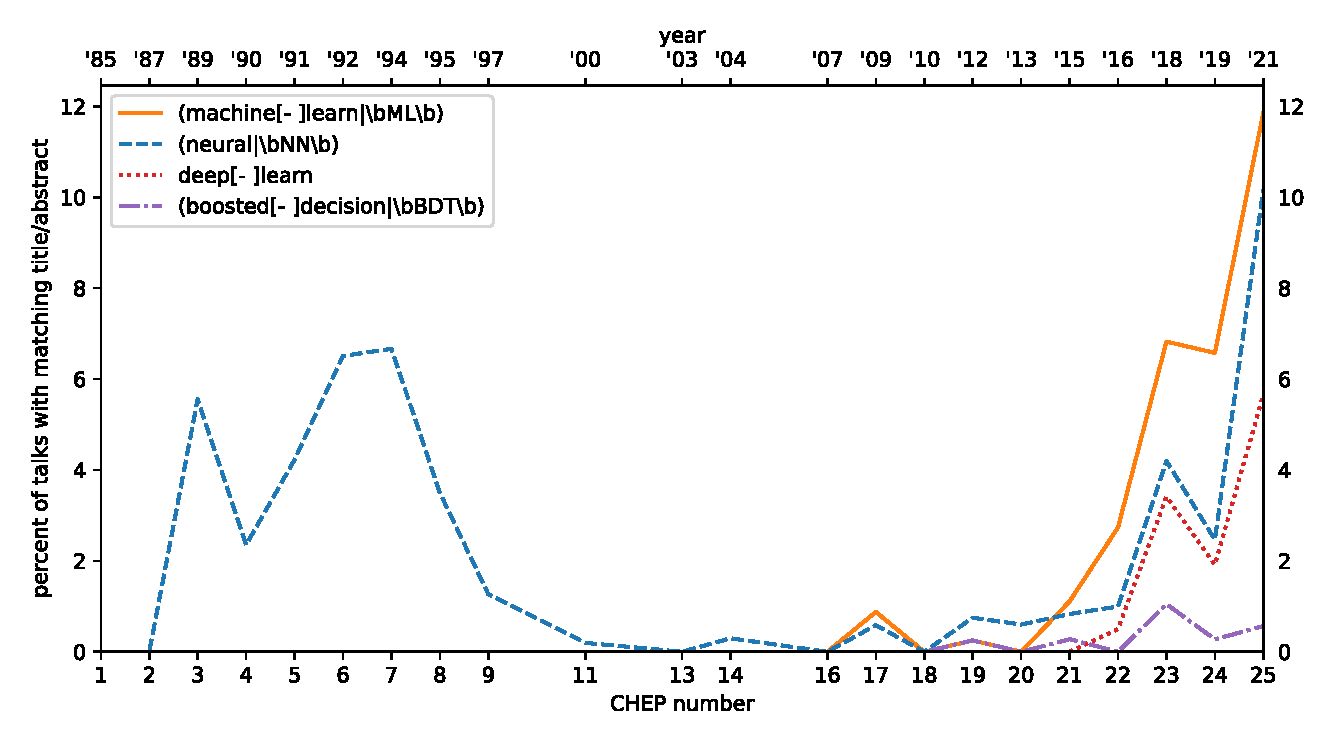
\includegraphics[width=0.95\linewidth]{PLOTS/chep-papers-ml.pdf}}\only<2>{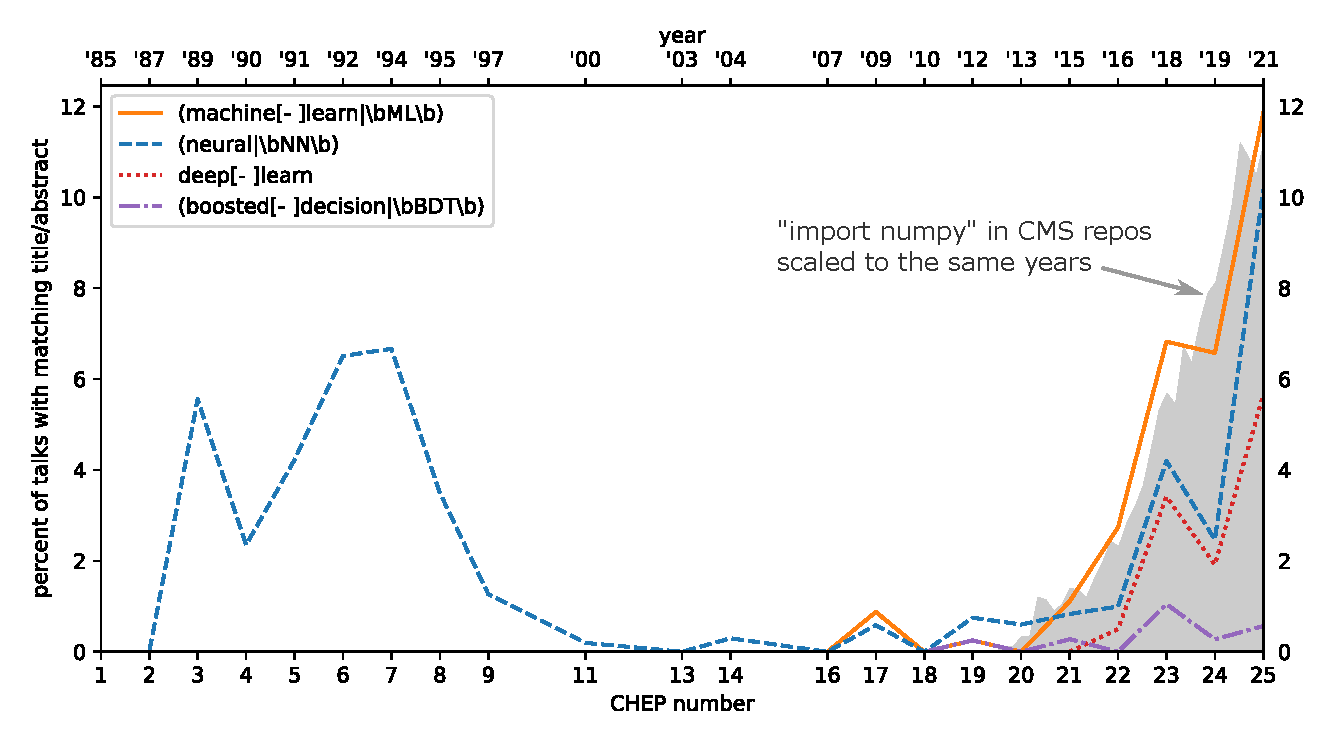
\includegraphics[width=0.95\linewidth]{PLOTS/chep-papers-ml-explained.pdf}}
\end{center}
\end{frame}

\begin{frame}{PyHEP 2020 survey}
\vspace{0.5 cm}
\begin{columns}
\column{1.1\linewidth}
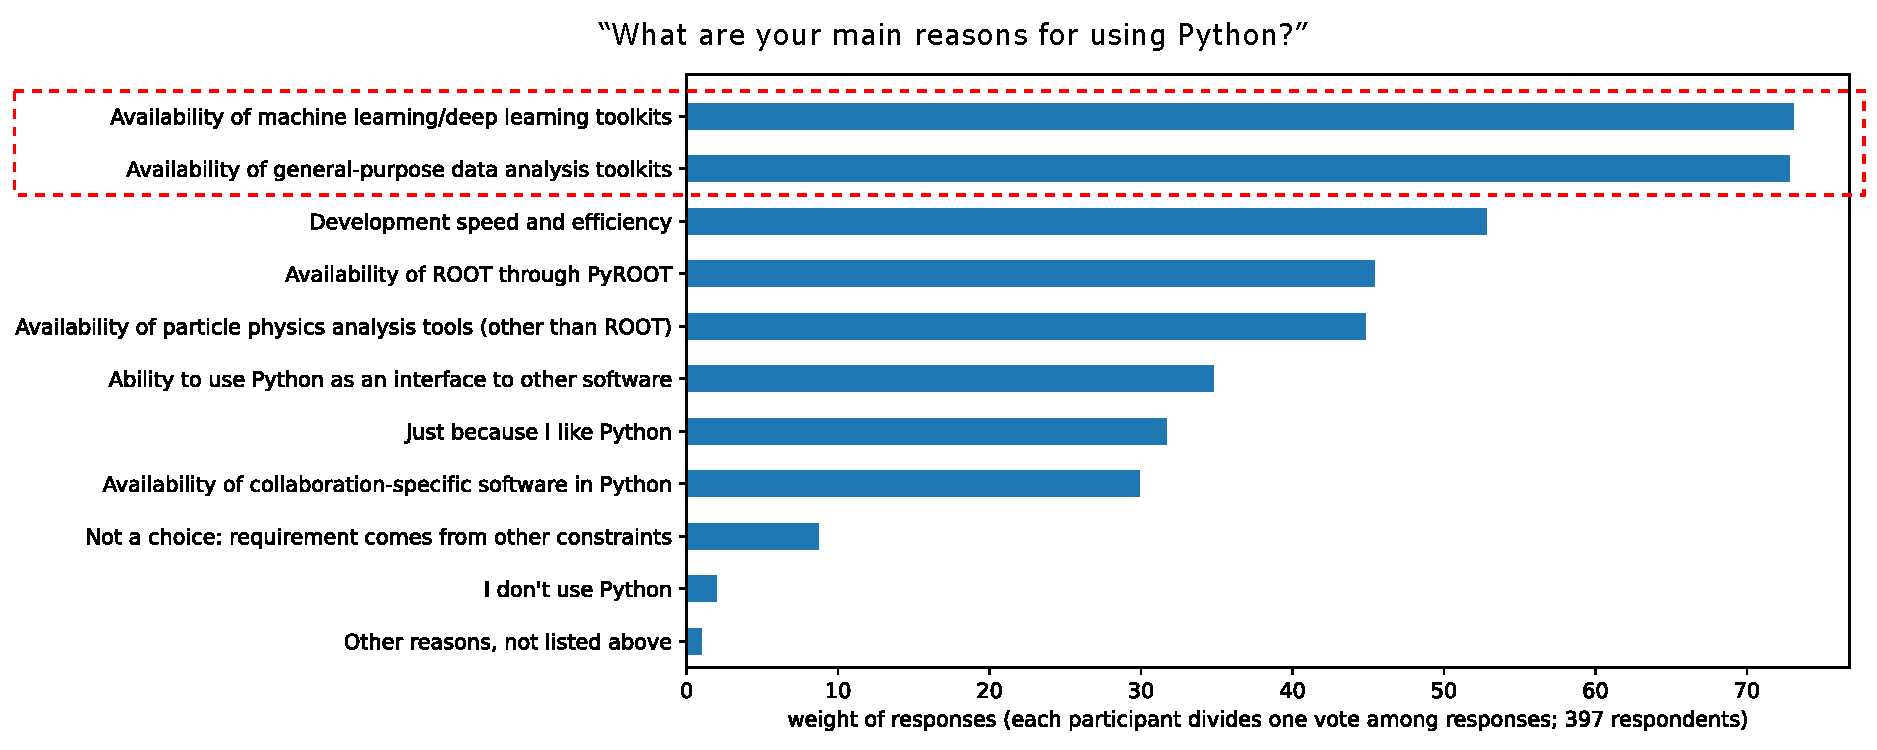
\includegraphics[width=\linewidth]{PLOTS/pyhep2020-why-use-python.pdf}
\end{columns}
\end{frame}

\begin{frame}{\mbox{ }}
\Large
Probably prompted by outside developments in machine learning, particle physicists are now mixing tools from other fields into their analyses.
\end{frame}

\begin{frame}{But they are using C++ {\it and} Python, ROOT {\it and} other toolkits}
\vspace{0.25 cm}
Again, from the PyHEP 2020 survey ($N = 406$):

\begin{columns}
\column{1.1\linewidth}
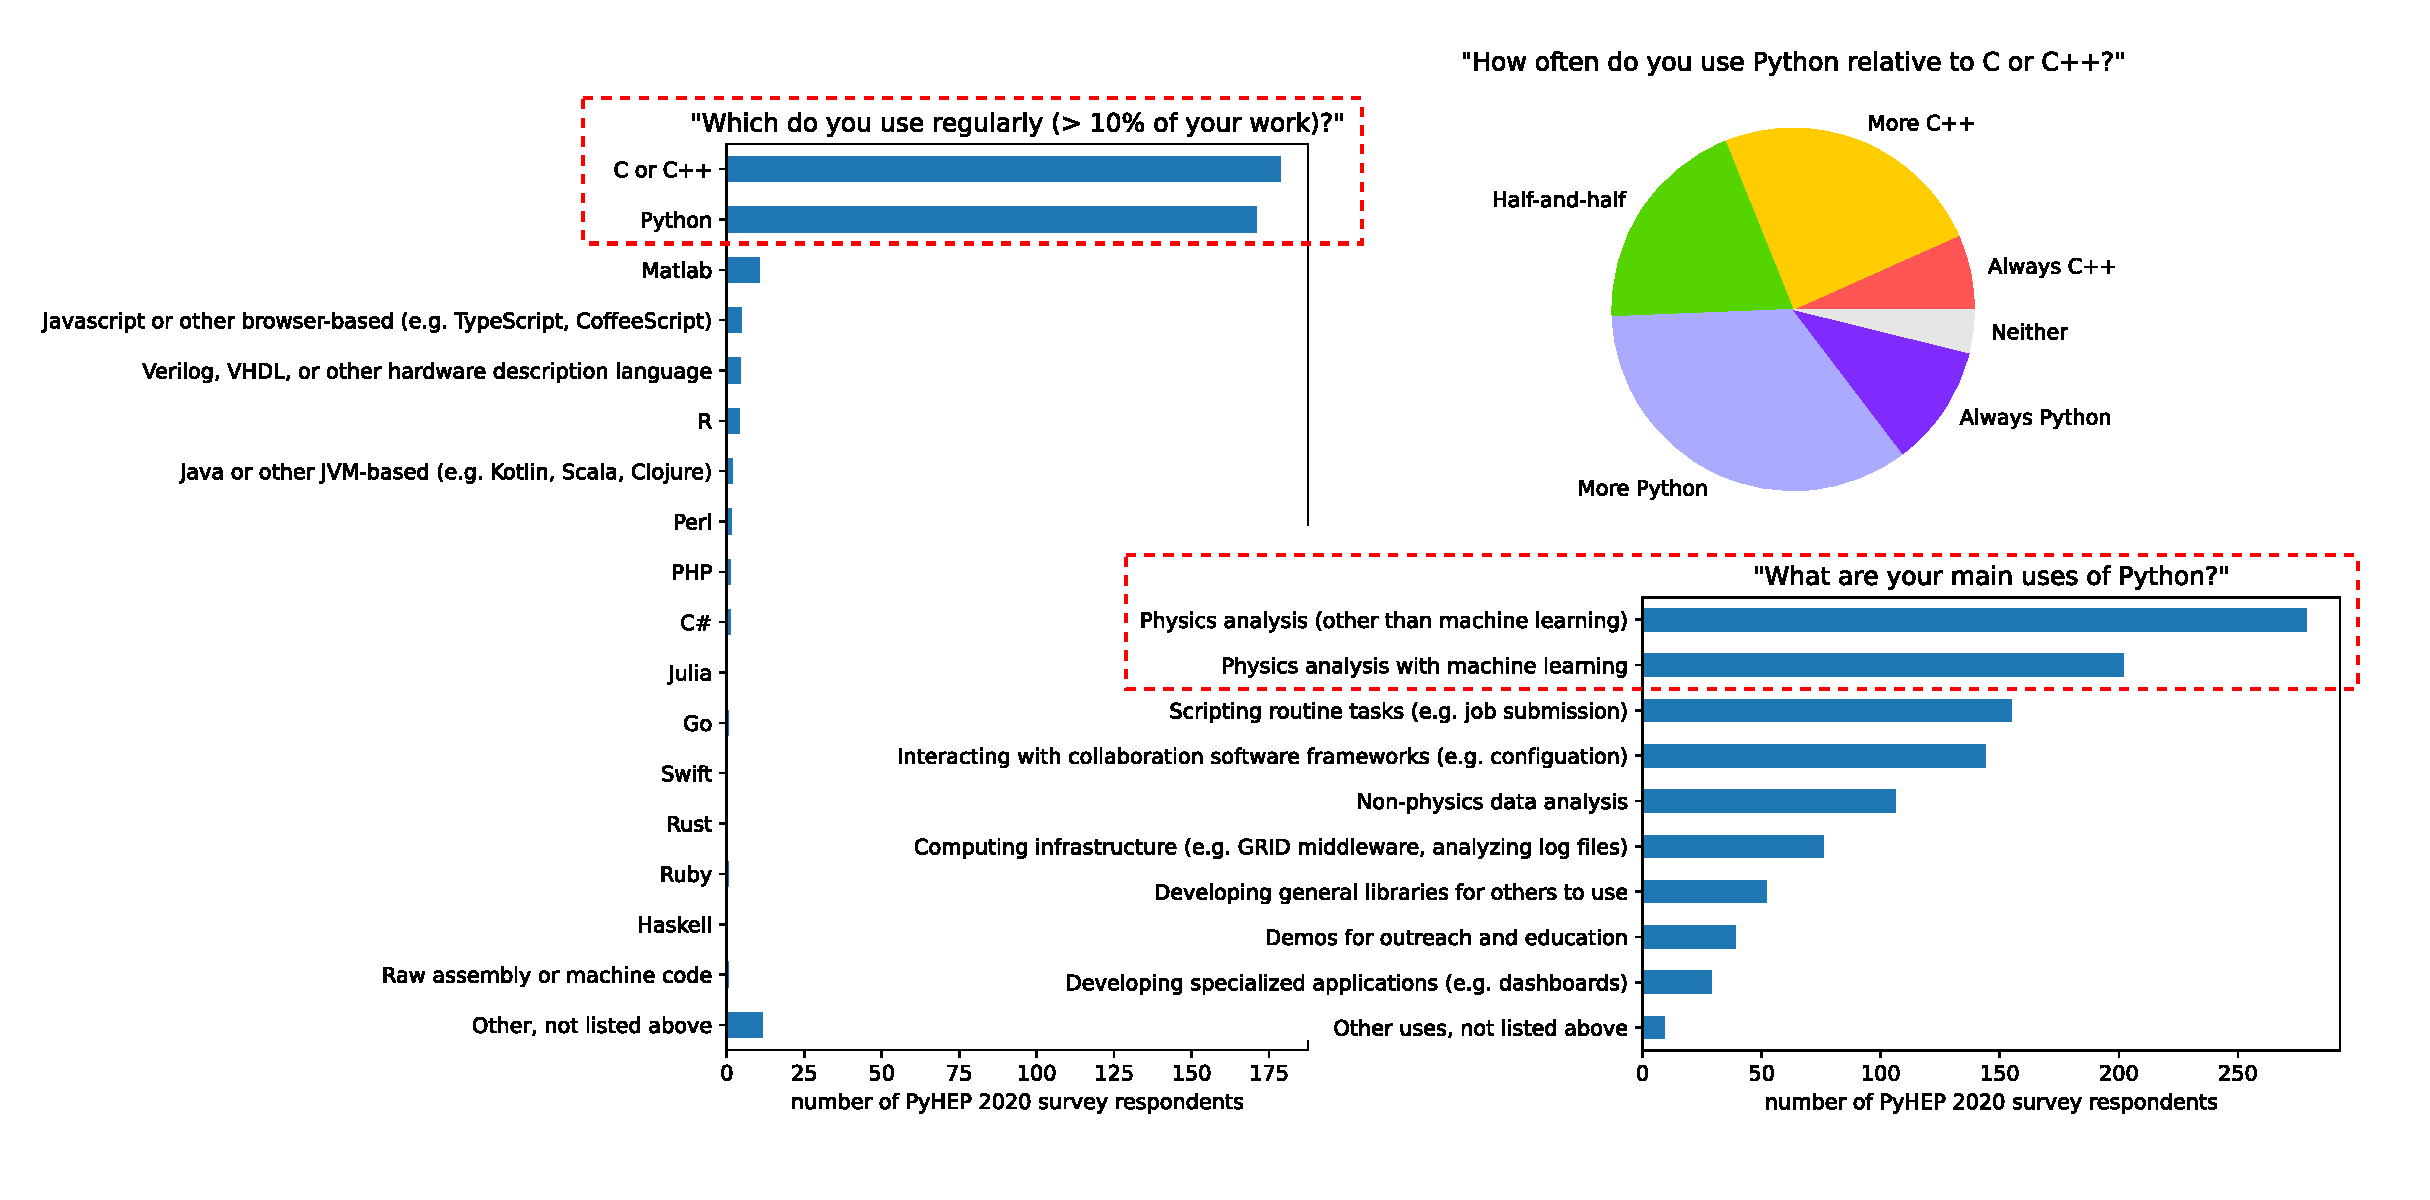
\includegraphics[width=\linewidth]{PLOTS/pyhep2020-survey-5.pdf}
\end{columns}
\end{frame}

\begin{frame}{Mood in the community is for inclusiveness, too}
\vspace{0.5 cm}
\begin{columns}
\column{1.05\linewidth}
From the PyHEP 2022 Slack:

\vspace{0.15 cm}
\begin{itemize}\setlength{\itemsep}{0.25 cm}
\item ``Is the scikit-hep collection already a complete replacement for the traditional ROOT approach? \ldots\ I would love to mostly avoid ROOT.''

\item ``The goal is not to replace ROOT but to provide alternative analysis styles that can be complimentary for the work you want to do. So I don't think anyone wants to try to reimpliment {\it everything} ROOT does, but LHCb has done an entire analysis using only Scikit-HEP tools: \textcolor{blue}{\url{https://inspirehep.net/literature/1889335}}

\textcolor{blue}{\url{https://indico.cern.ch/event/1126109/contributions/4780169}}''

\item ``But let me stress is once more as these matters come often. The whole ecosystem can do a lot in various ways, and indeed ROOT and Scikit-HEP take different routes/philosophies. But they are alternative approaches, not replacements. In the end we all win by having several approaches/packages.''
\end{itemize}

\vspace{0.25 cm}
(Lots of eyeballs, hearts, thumbs-up, smiles, etc.)
\end{columns}
\end{frame}

\begin{frame}{PyHEP talks about connecting ROOT-based systems to others}
\vspace{0.5 cm}

\begin{itemize}\setlength{\itemsep}{0.35 cm}
\item Uhepp: Sharing plots in a self-contained format \hfill \textcolor{gray}{Frank Sauerburger}
\item Lessons learned converting a production-grade Python CMS analysis to distributed RDataFrame \hfill \textcolor{gray}{Tommaso Tedeschi and Vincenzo Padulano}
\item Awkward RDataFrame Tutorial \hfill \textcolor{gray}{Ianna Osborne}
\item Enabling Dask Interoperability with XRootD Storage Systems \hfill \textcolor{gray}{Scott Demarest}
\item Using C++ From Numba, Fast and Automatic \hfill \textcolor{gray}{Baidyanath Kundu}
\item Pyhf to Combine Converter \hfill \textcolor{gray}{Petey Ridolfi}
\end{itemize}

\vspace{0.5 cm}
(Not counting talks about ROOT and HepMC3 {\it files}, Minuit, Pythia, and others.)
\end{frame}

\begin{frame}{\mbox{ }}
\Large
But that doesn't mean that we {\it avoid} overlaps with ROOT or {\it only} bridge ROOT functionality to the outside world.

\vspace{1 cm}
\begin{uncoverenv}<2->
We add particle physics functionality to the scientific Python ecosystem in a Pythonic way:

\begin{itemize}
\item<3-> following Python conventions and practices (as they evolve)
\item<4-> share data between packages by referencing arrays
\item<5-> preference for small-scoped, cooperating packages
\end{itemize}
\end{uncoverenv}
\end{frame}

\begin{frame}{This is our model: pieces that can be plugged together}
\vspace{0.75 cm}
\Large

\begin{columns}
\column{0.55\linewidth}
\begin{uncoverenv}<1->
\mbox{ } \hfill Scientific Python ecosystem \hfill \mbox{ }

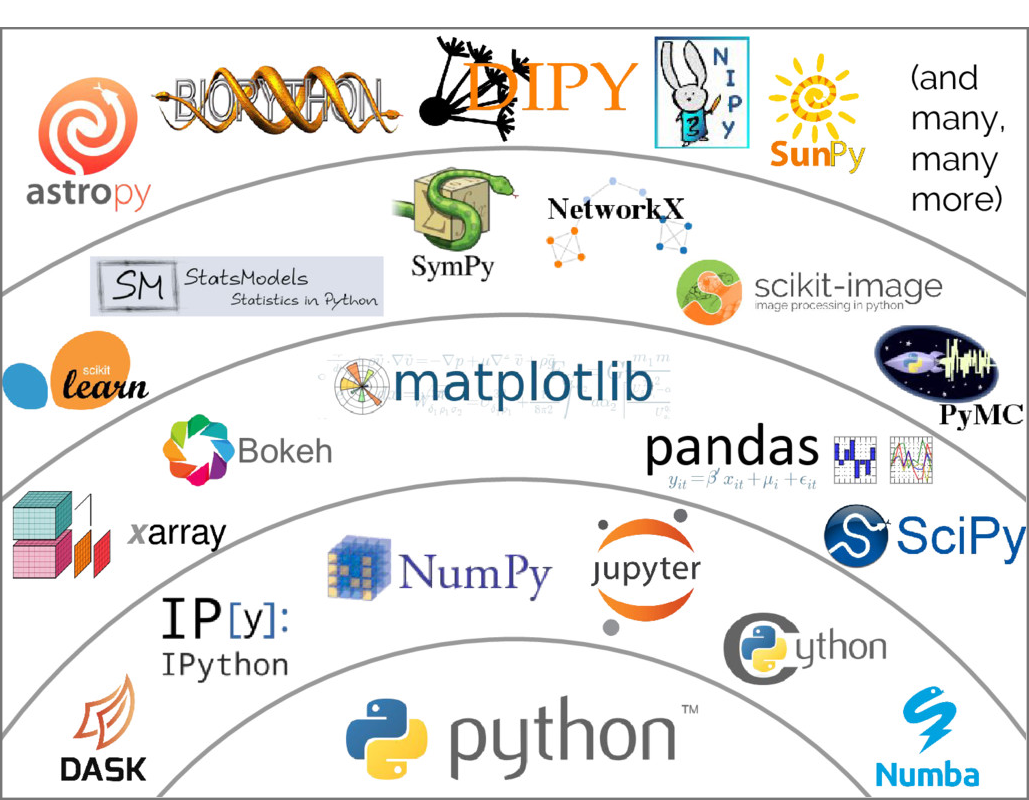
\includegraphics[width=\linewidth]{PLOTS/shells-border.png}
\end{uncoverenv}

\column{0.55\linewidth}
\begin{uncoverenv}<2->
\mbox{ } \hfill Scikit-HEP ecosystem \hfill \mbox{ }

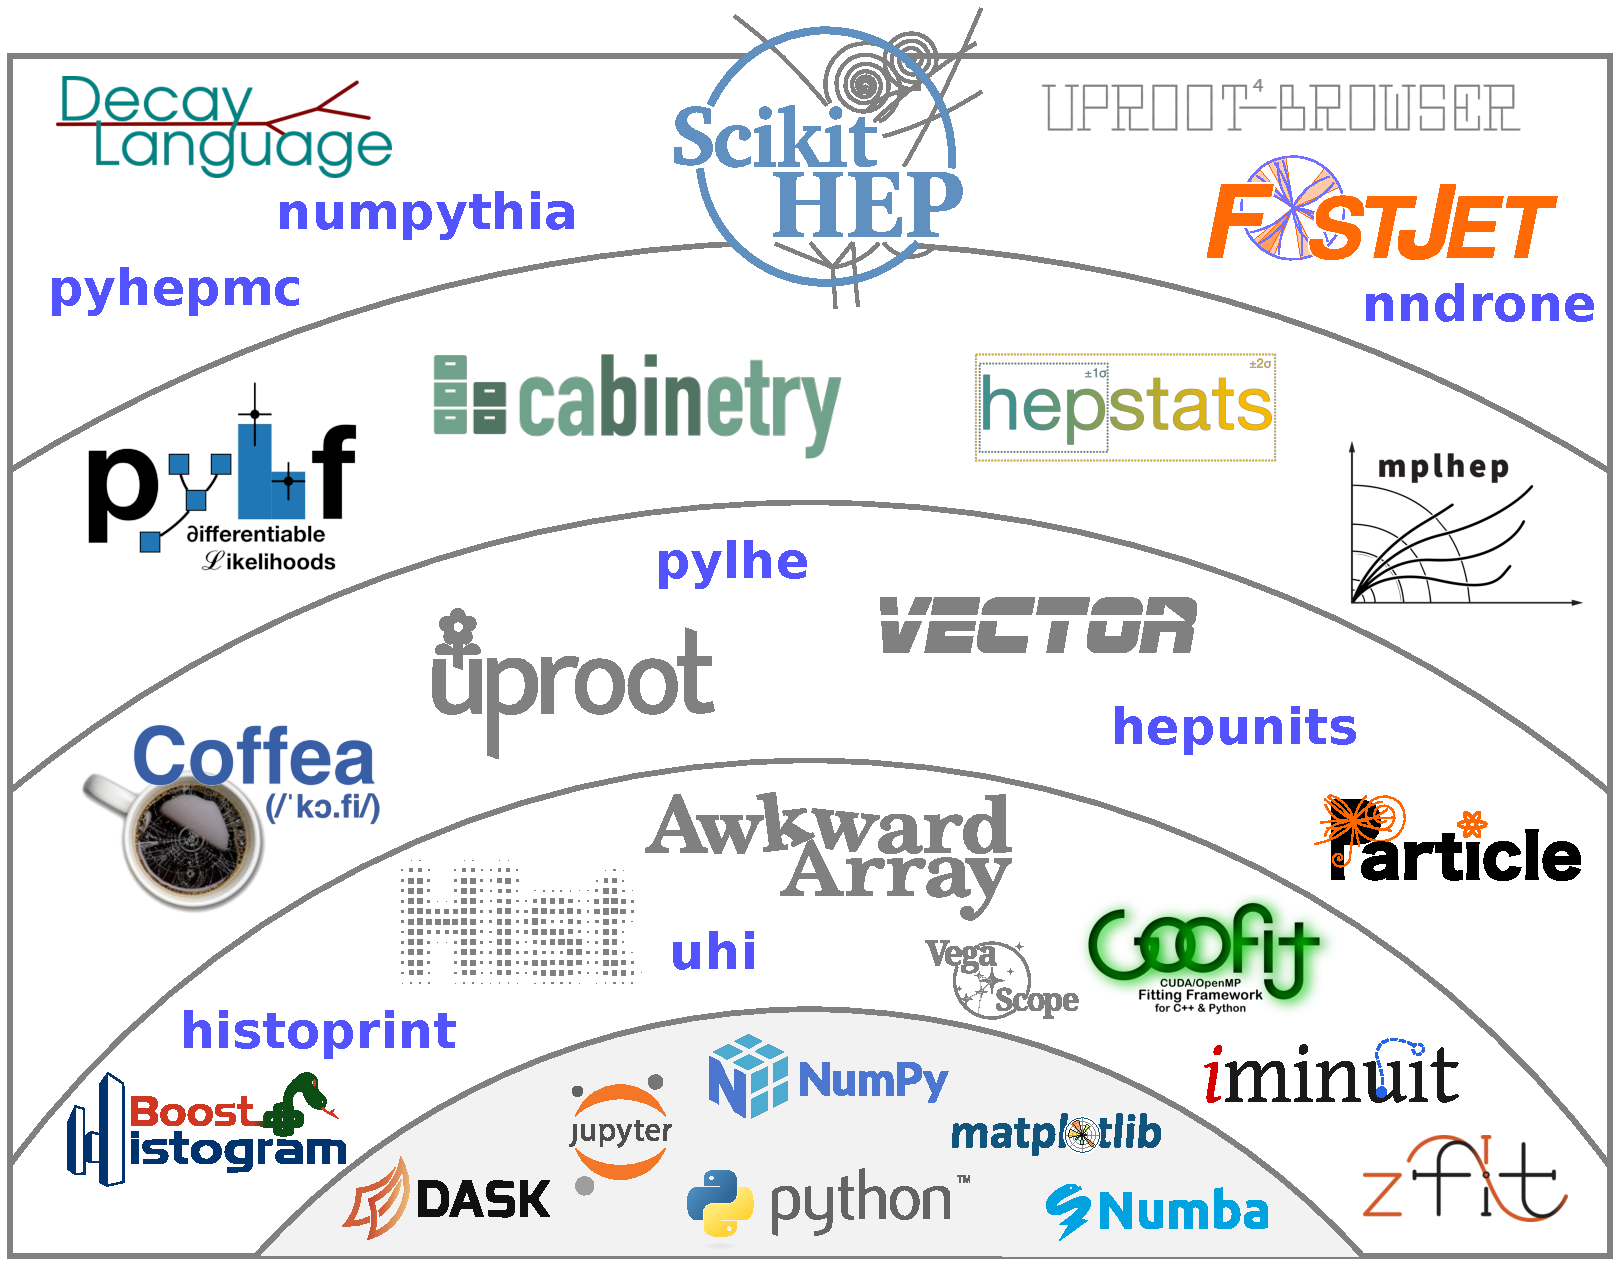
\includegraphics[width=\linewidth]{PLOTS/shells-hep.pdf}
\end{uncoverenv}
\end{columns}
\end{frame}

\begin{frame}{Since we started, packages grew in popularity {\it and number}}
\vspace{0.35 cm}

Download rates of Scikit-HEP packages (on Mac \& Windows: no batch jobs)

\only<1>{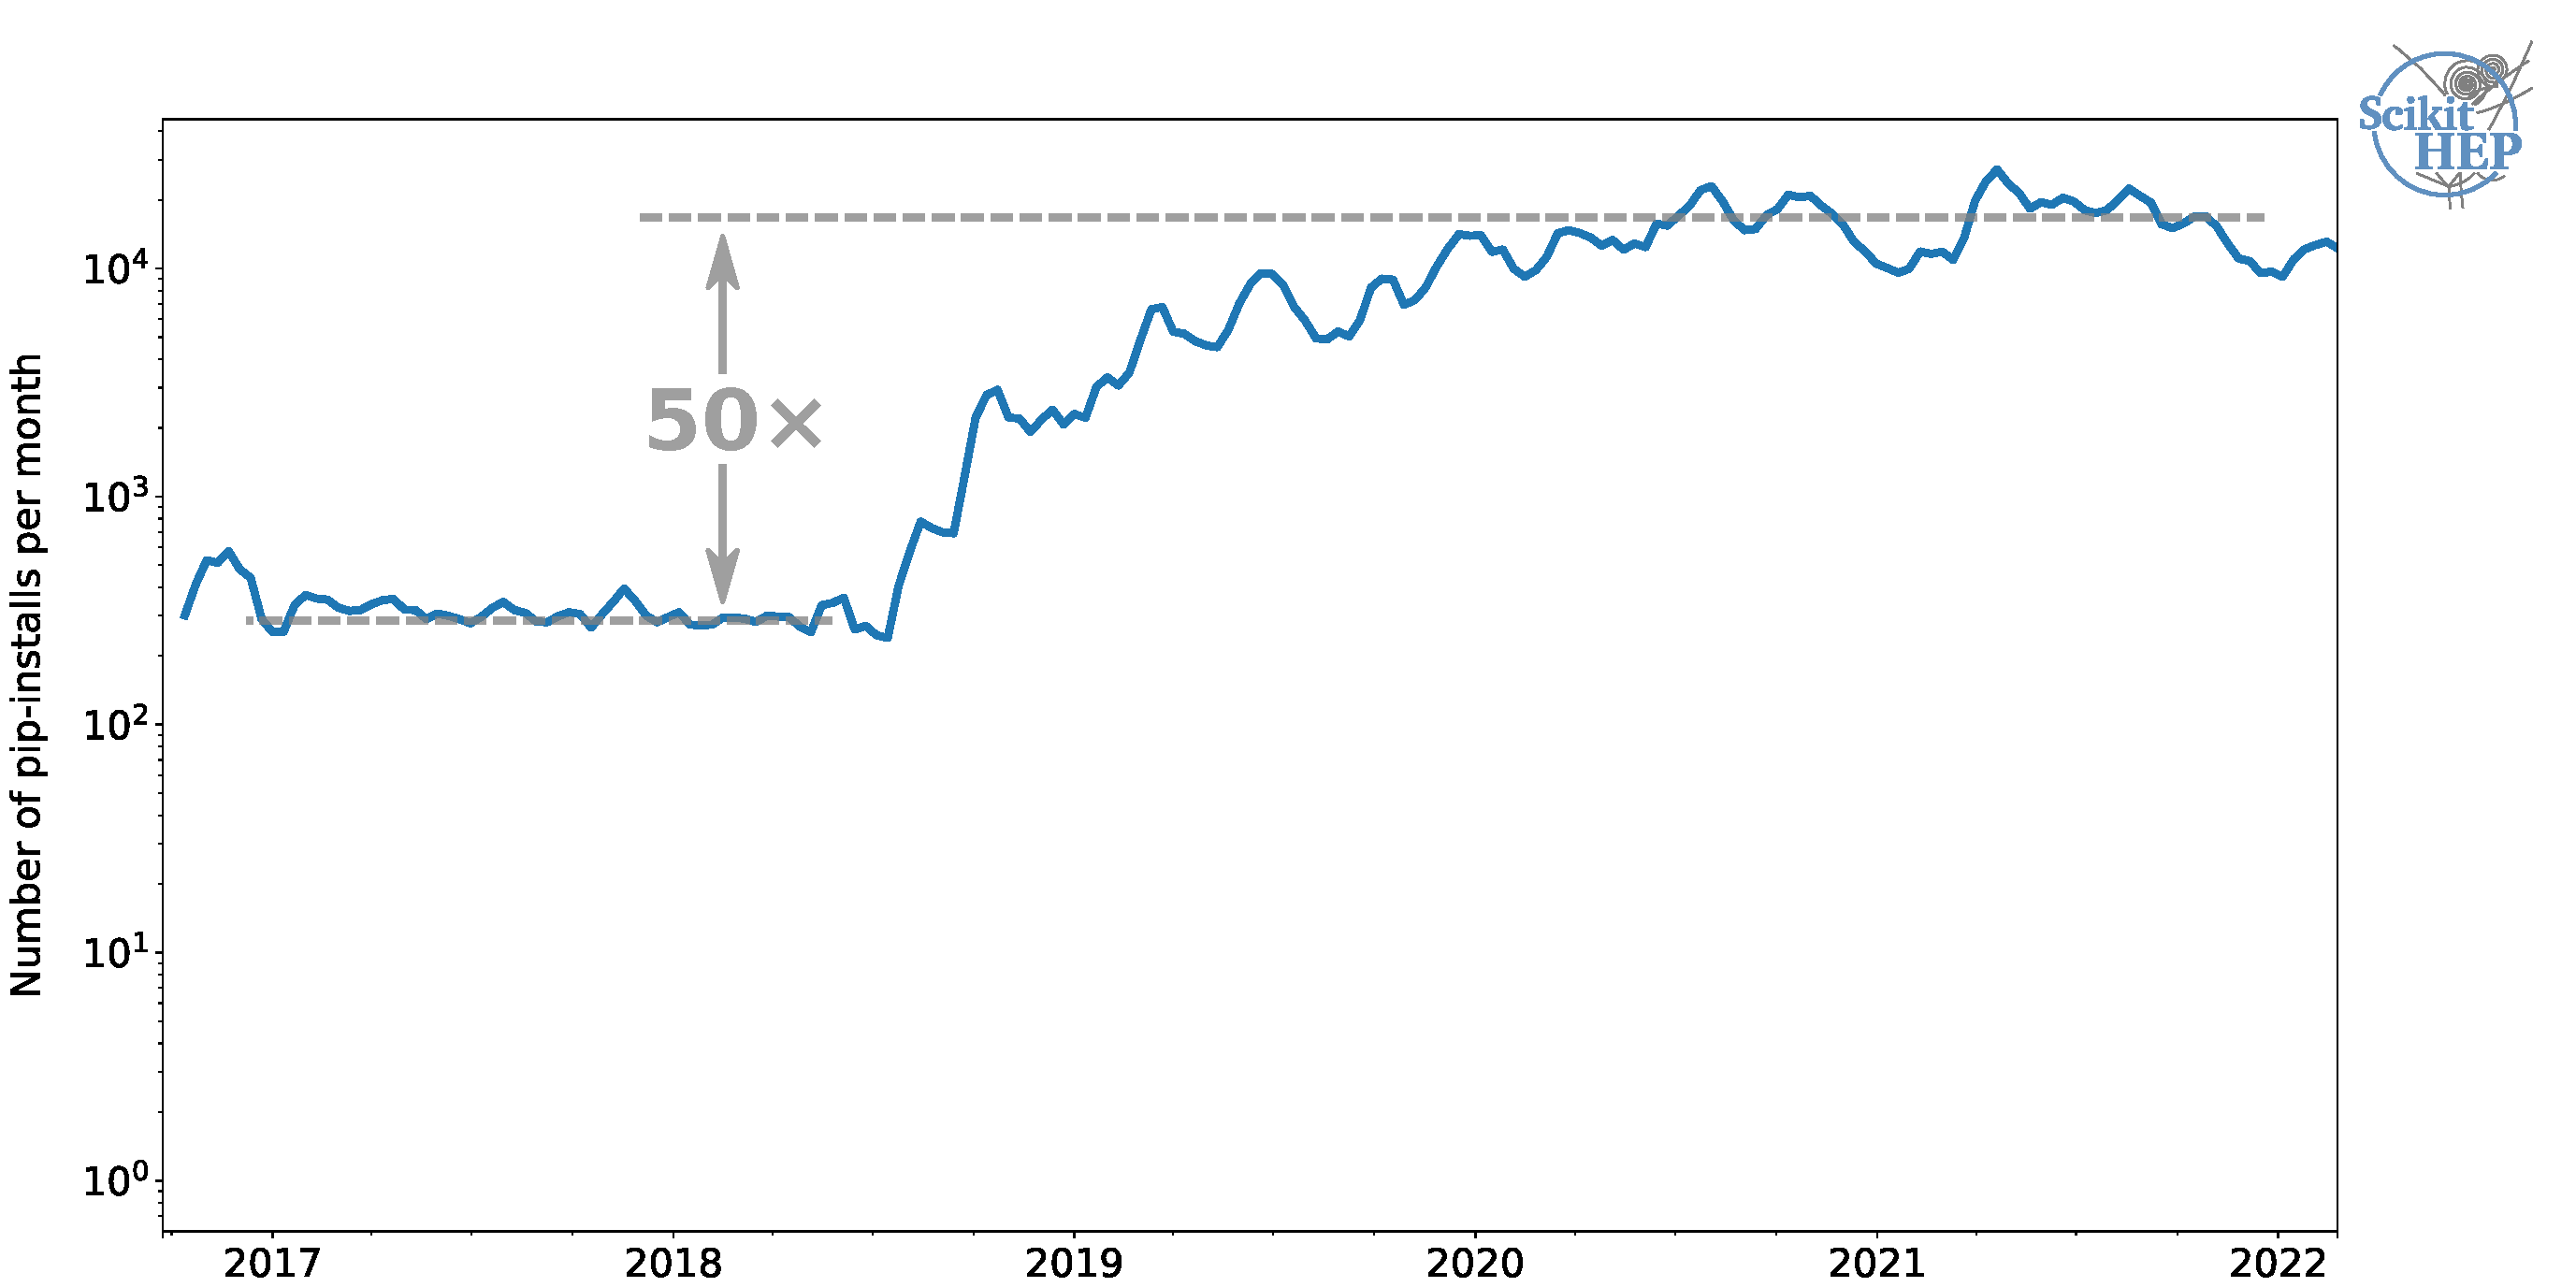
\includegraphics[width=\linewidth]{PLOTS/pip-macwin-scikithep-log-for-report-0.pdf}}\only<2>{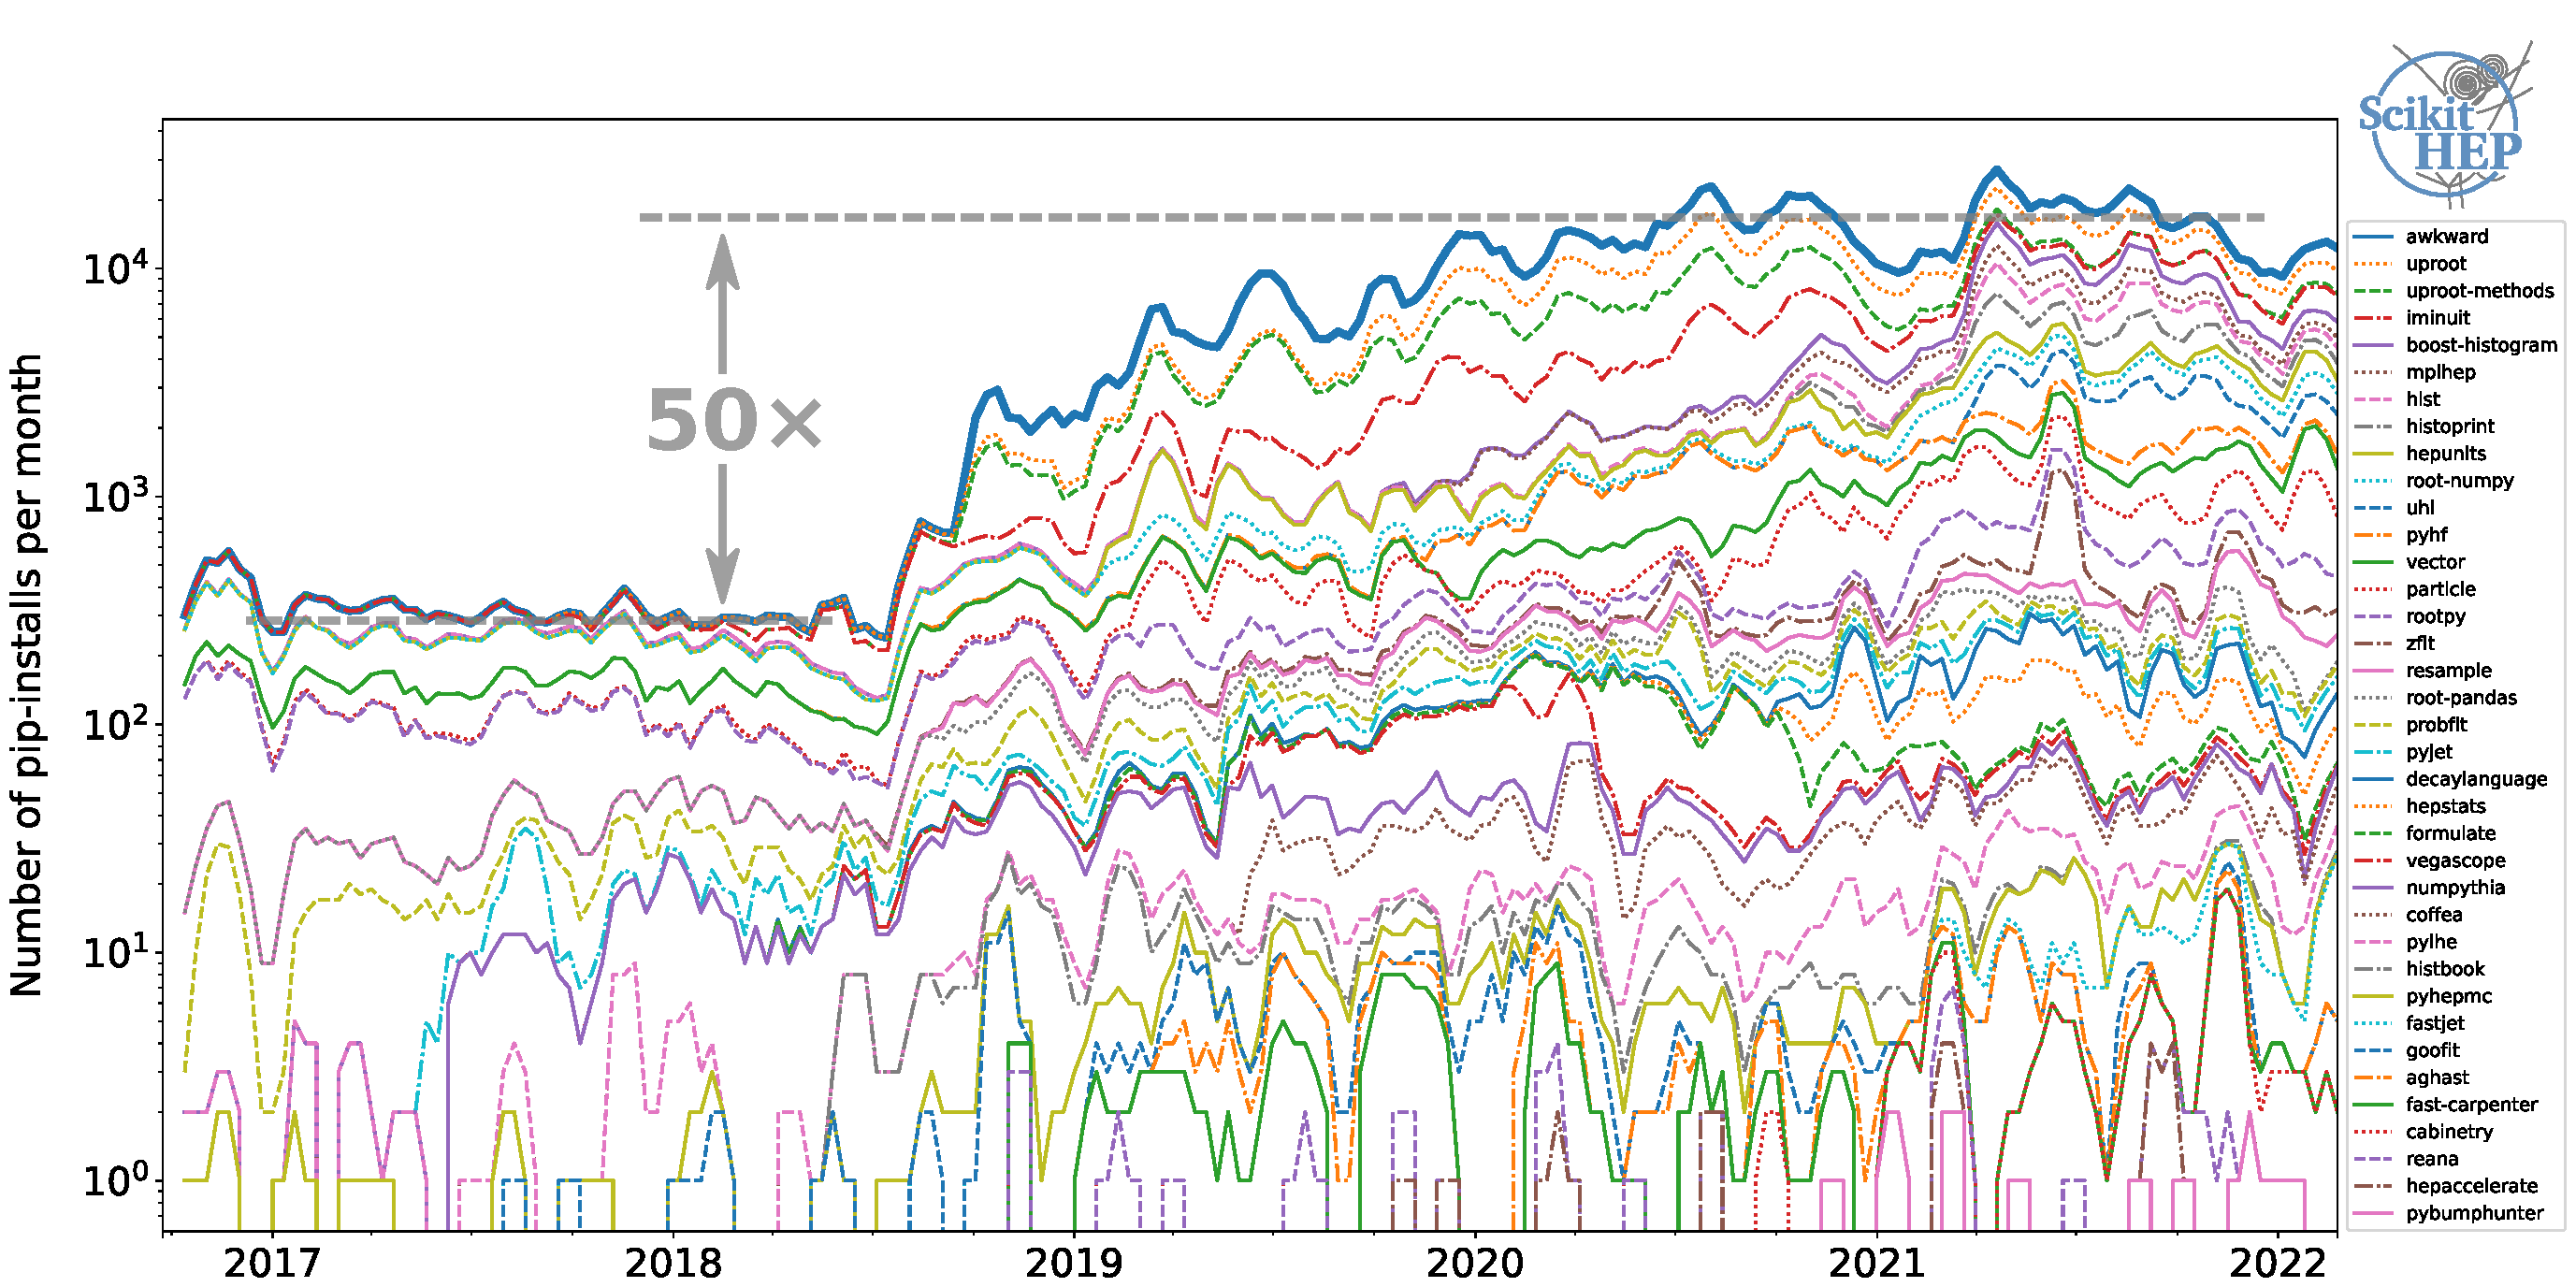
\includegraphics[width=\linewidth]{PLOTS/pip-macwin-scikithep-log-for-report.pdf}}
\end{frame}

\begin{frame}{\mbox{ }}
\begin{columns}[t]
\column{0.5\linewidth}
\underline{\large Advantages of small packages}

\vspace{0.2 cm}
\begin{itemize}
\item<2-> Agile: when a new area needs to be filled or an old package ceases to be maintained/liked, a new one can move in without historical constraints.

\item<3-> Recognition: author of that package is highly visible.

\item<4-> Prevents scope-creep: pressure for features outside the target area can be refused without guilt.

\end{itemize}

\column{0.5\linewidth}
\underline{\large Disadvantages of small packages}

\vspace{0.2 cm}
\begin{itemize}
\item<5-> Coordination: what if no one wants to cover a given target area?

\item<6-> Coordination: what if everyone wants to cover the same target area?

\item<7-> Coordination: what if packages in neighboring target areas can't share data?

\item<8-> Communication: where do users get help solving problems that cross target areas?
\end{itemize}

\end{columns}
\end{frame}

\begin{frame}{Case study showing the worst and the best: histograms}
\vspace{0.25 cm}
NumPy, Matplotlib, Pandas, etc.\ can plot histograms, but not the way we need in particle physics: as fillable objects, with (negative) weights, error propagation, \ldots

\vspace{0.5 cm}
\uncover<2->{So we need to make our own histogram package. And it seems easy, right?}

\vspace{0.5 cm}
\uncover<3->{Physicists have created at least 20 histogram packages in Python, mostly single-author.}

\vspace{0.5 cm}
\begin{uncoverenv}<3->
\begin{columns}
\scriptsize
\column{0.26\linewidth}
\begin{itemize}
\item PyROOT (2004--now)
\item PAIDA (2004--2007)
\item Plothon (2007--2008)
\item SVGFig (2008--2009)
\item YODA (2008--now)
\end{itemize}

\column{0.27\linewidth}
\begin{itemize}
\item DANSE (2009--2011)
\item rootpy (2011--2019)
\item SimpleHist (2011--2015)
\item pyhistogram (2015)
\item multihist (2015--now)
\end{itemize}

\column{0.28\linewidth}
\begin{itemize}
\item matplotlib-hep (2016)
\item QHist (2017--2019)
\item Physt (2016--now)
\item \mbox{Histogrammar (2016--now)\hspace{-0.2 cm}}
\item HistBook (2018--2019)
\end{itemize}

\column{0.32\linewidth}
\begin{itemize}
\item Coffea.hist (2019--2022)
\item boost-histogram (2019--now)
\item mplhep (2019--now)
\item histoprint (2020--now)
\item hist (2020--now)
\end{itemize}

\end{columns}
\end{uncoverenv}
\end{frame}

\begin{frame}[fragile]{In Scikit-HEP, several packages converged to work together}
\vspace{0.5 cm}
\begin{columns}
\column{0.6\linewidth}
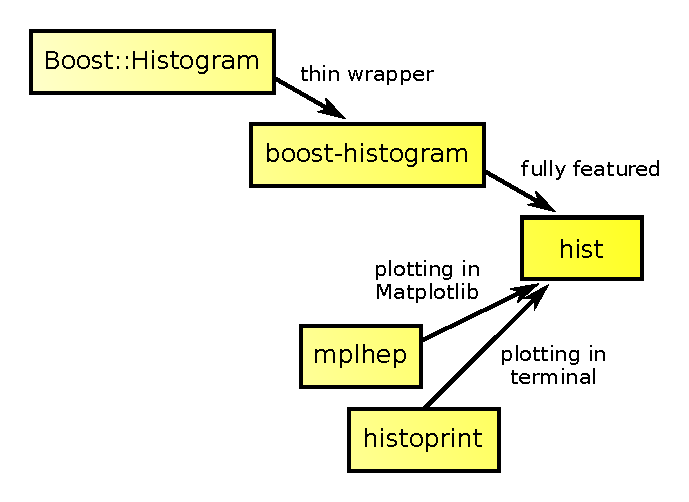
\includegraphics[width=\linewidth]{PLOTS/histogram-convergence.pdf}

\column{0.45\linewidth}
Originally, each of these was developed independently by a single author.

\vspace{0.75 cm}
\begin{uncoverenv}<2->
They each provide a piece of functionality users can get through

\begin{minted}{python}
import hist
\end{minted}
\end{uncoverenv}

\vspace{0.75 cm}
\uncover<3->{Now, 47 developers have contributed to these packages, and 20 contributed to more than one.}
\end{columns}
\end{frame}

\begin{frame}{Histogram proliferation and convergence}
\large
\vspace{0.25 cm}

Number of unique developers contributing to each package per month (in git). Measures concentration of {\it developer activity}, not users.

\vspace{0.1 cm}
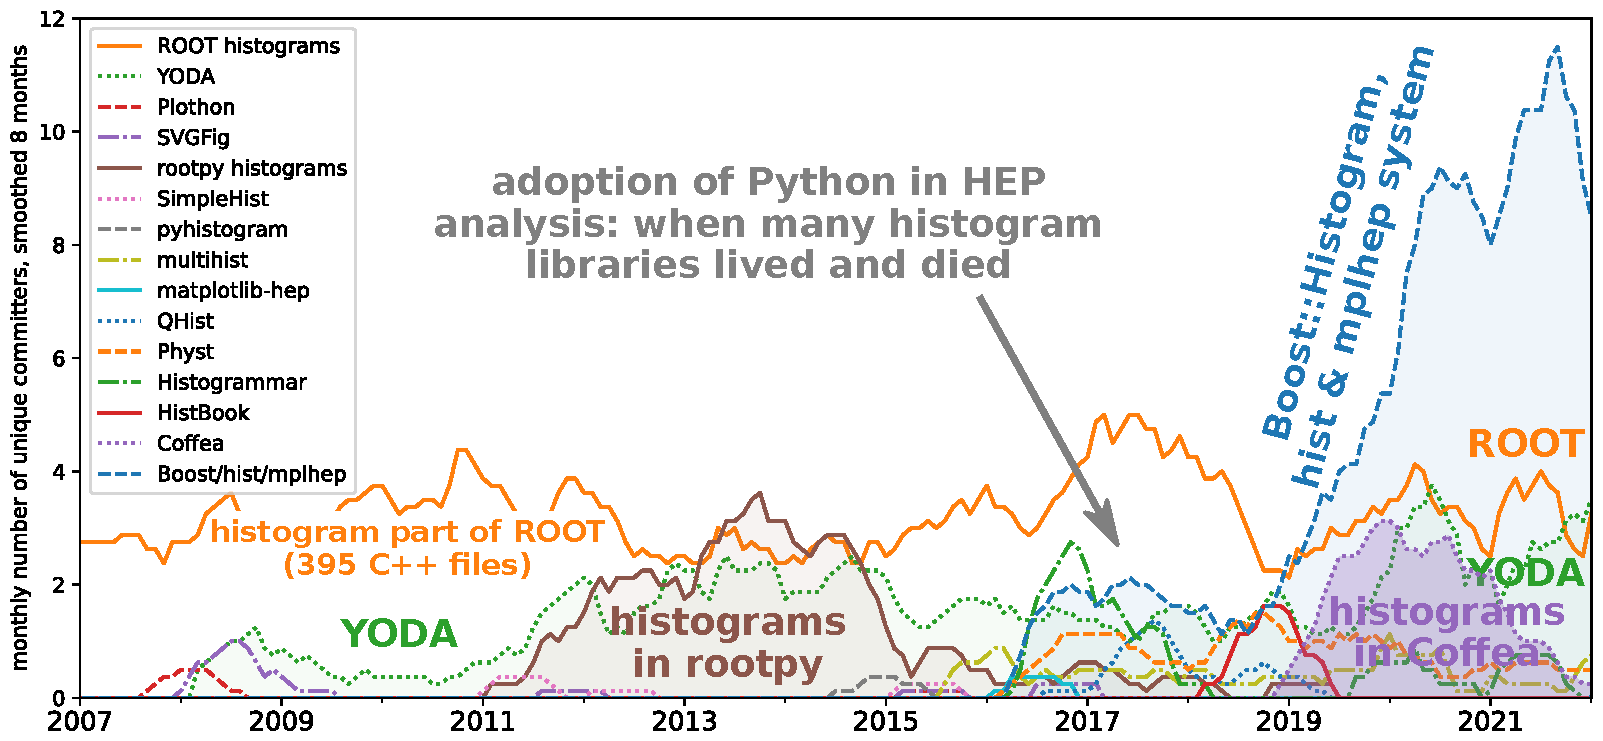
\includegraphics[width=\linewidth]{PLOTS/github-histogram-libraries.pdf}
\end{frame}

\begin{frame}{Now we define the interfaces: agreed-upon protocols}
\vspace{0.5 cm}
\begin{columns}
\column{1.1\linewidth}
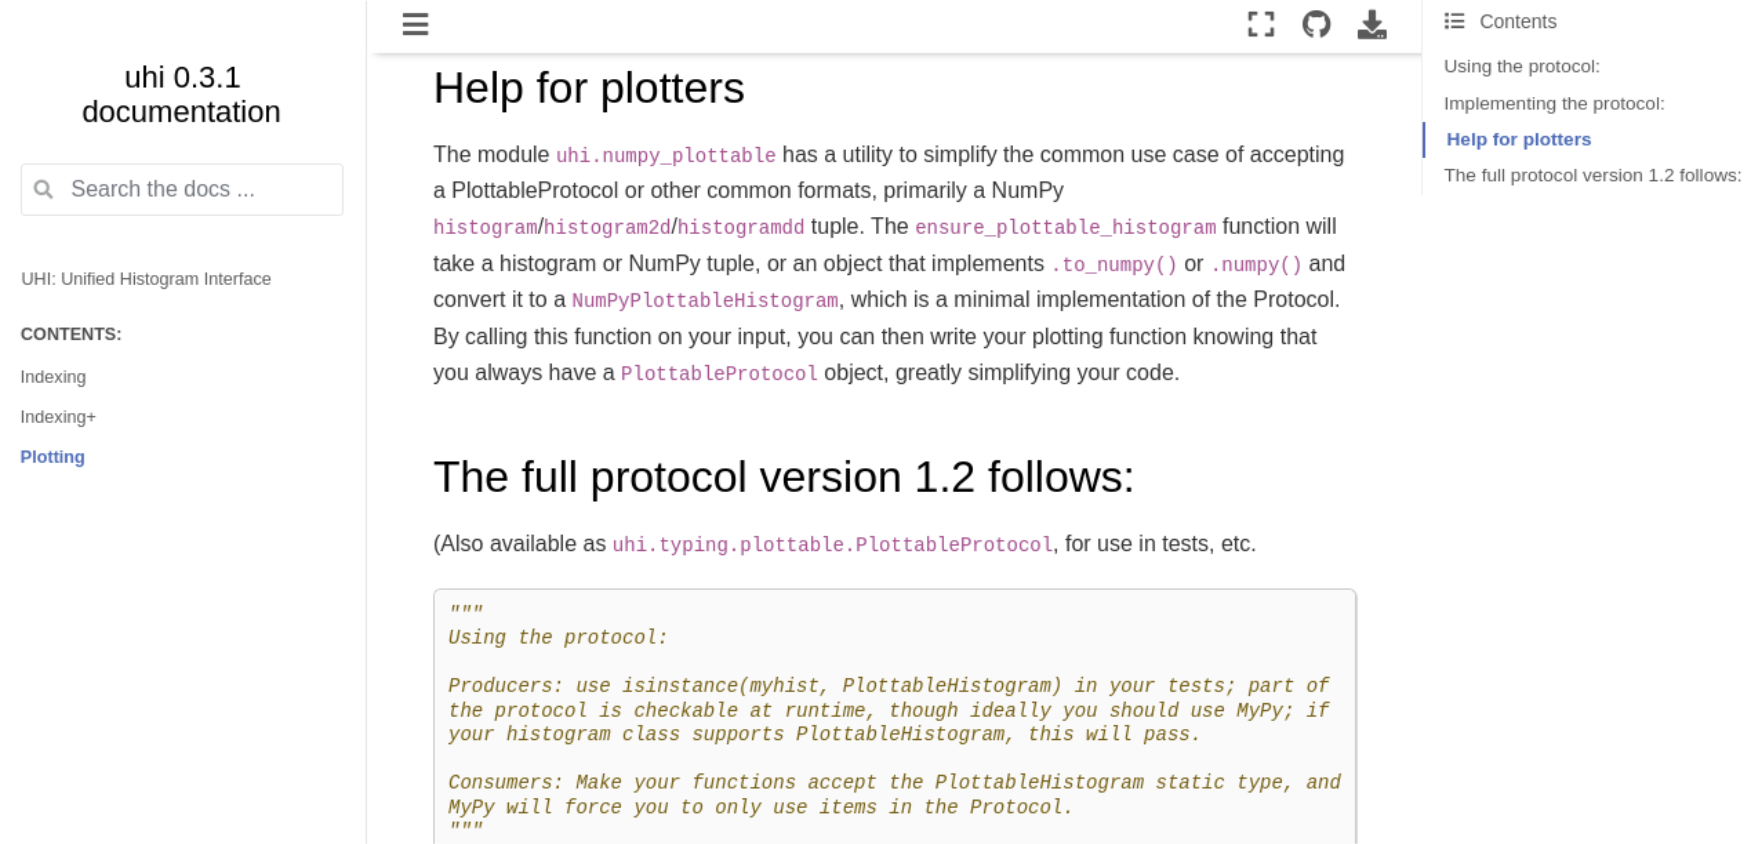
\includegraphics[width=\linewidth]{PLOTS/histogram-protocol-screenshot.png}
\end{columns}
\end{frame}

\begin{frame}{Addressing the disadvantages: developer coordination}
\vspace{0.25 cm}
IRIS-HEP Slack: $\sim$150 active members weekly, not all in IRIS-HEP, not all in HEP

\vspace{0.25 cm}
\begin{columns}
\column{1.1\linewidth}
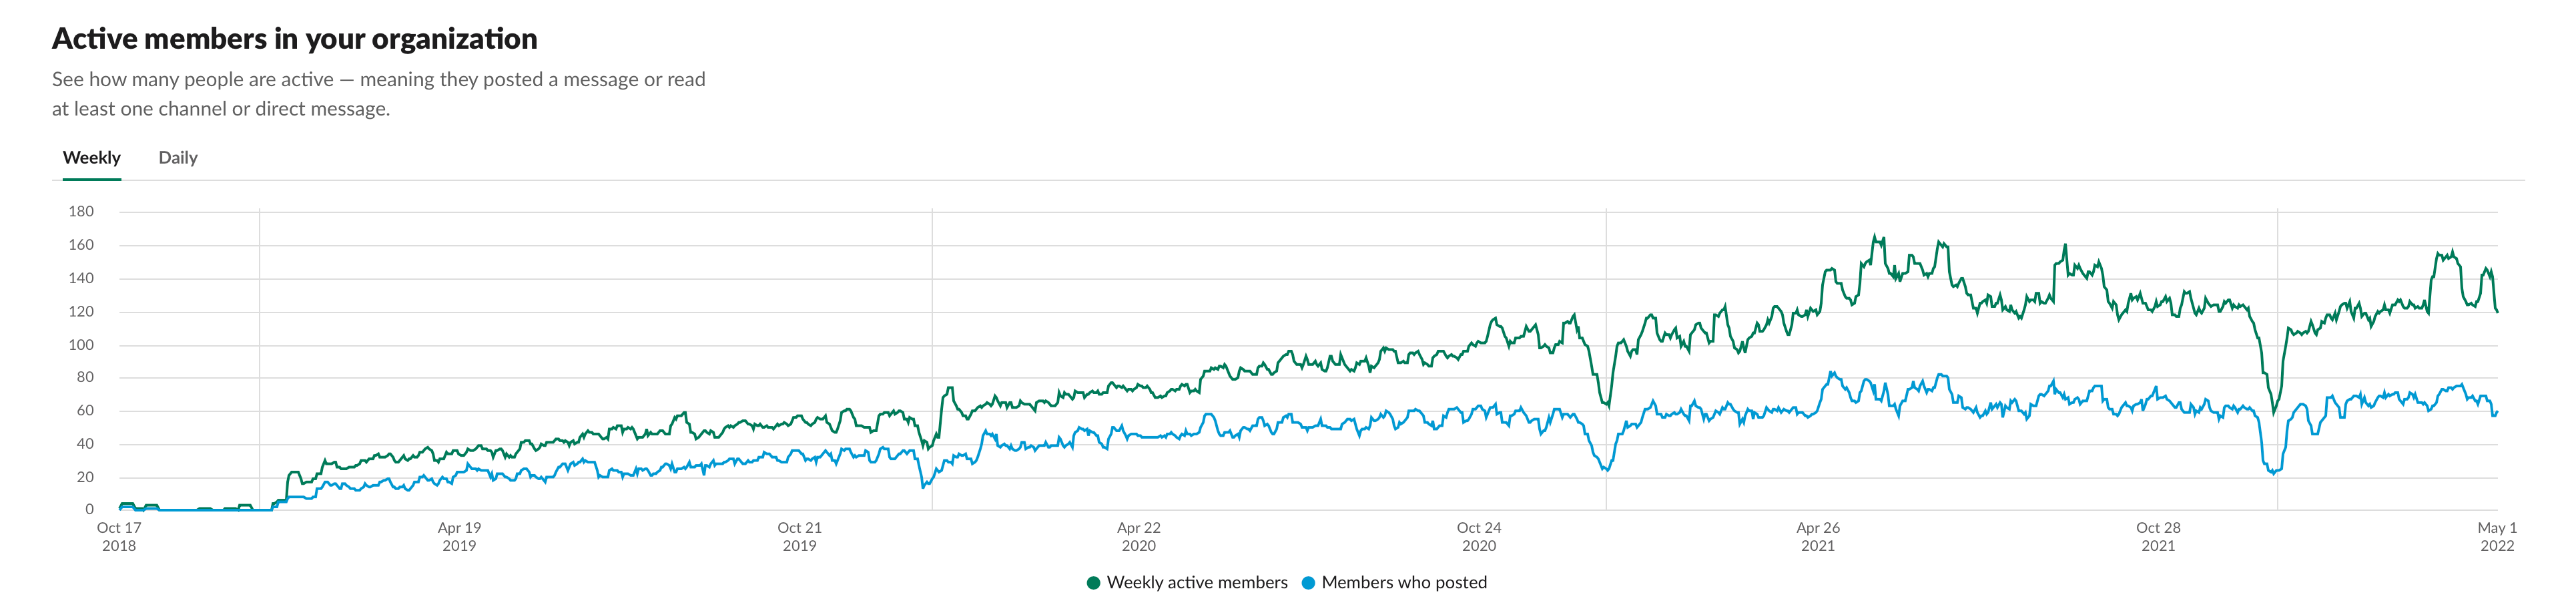
\includegraphics[width=\linewidth]{PLOTS/20220504-iris-hep-slack-analytics-members.png}
\end{columns}

\vspace{0.75 cm}
GitHub: also very active.

\vspace{0.25 cm}
I need a visualization that demonstrates not just the volume, but the ``off-diagonal'' interactions between developers of different packages and between the particle physics community and the wider community.
\end{frame}

\begin{frame}{Addressing the disadvantages: integration testing at scale}
\vspace{0.4 cm}
\begin{columns}
\column{1.1\linewidth}
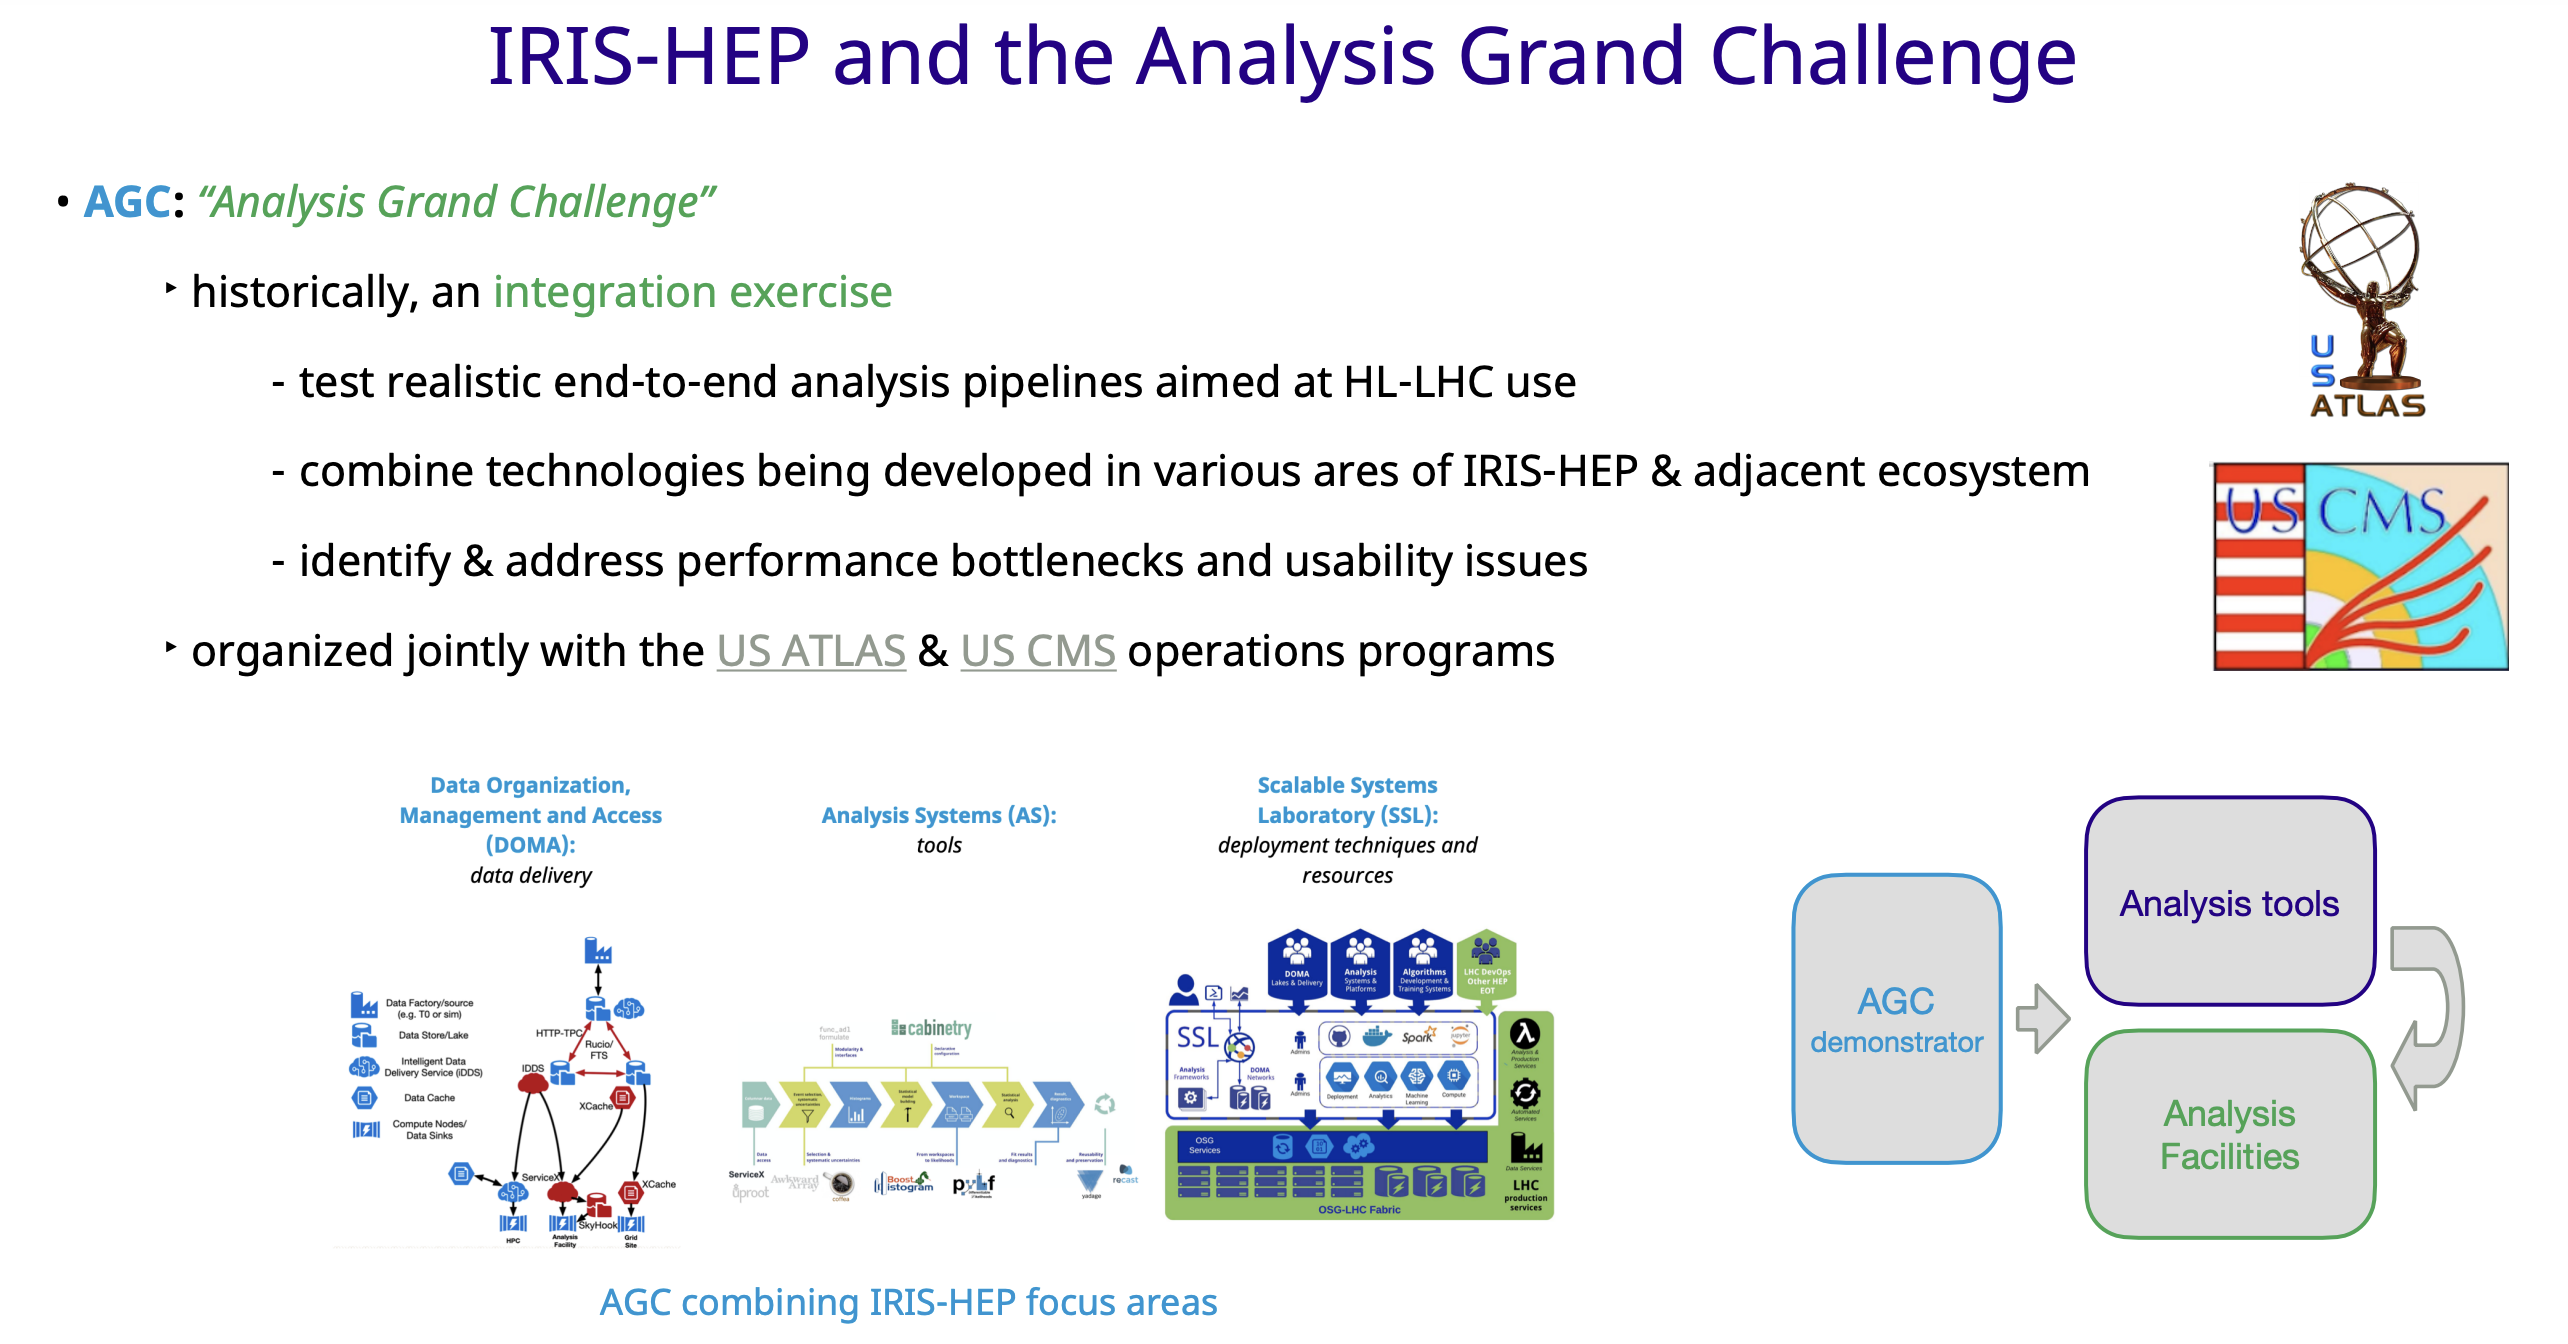
\includegraphics[width=\linewidth]{PLOTS/agc-slide.png}
\end{columns}
\end{frame}

\begin{frame}{Addressing the disadvantages: user communication}
\vspace{0.25 cm}
The problem is that we have {\it too many} ways to answer questions from users.

\vspace{0.25 cm}
\begin{itemize}
\item \textcolor{darkblue}{GitHub issues and discussions:} best so far, but distributed per-package
\item \textcolor{darkblue}{Gitter:} low-barrier chat, but also per-package
\item \textcolor{darkblue}{Mattermost:} CERN credentials are a barrier, but most LHC experiments are here
\item \textcolor{darkblue}{Slack:} required invitation is a barrier; mostly developers, anyway
\item \textcolor{darkblue}{StackOverflow:} good for cross-package discussions, but too diffuse in non-scientific world (when non-physicists answer questions, they're usually wrong)
\item \textcolor{darkblue}{Scientific-Python.org Discourse and Discord:} options under consideration
\end{itemize}

\vspace{0.5 cm}
We would benefit by converging on one and sending users to that single forum.
\end{frame}

\begin{frame}{PyHEP workshop evolved from developer-focus to user-focus}
\Large
\vspace{0.35 cm}

\begin{columns}
\column{0.5\linewidth}
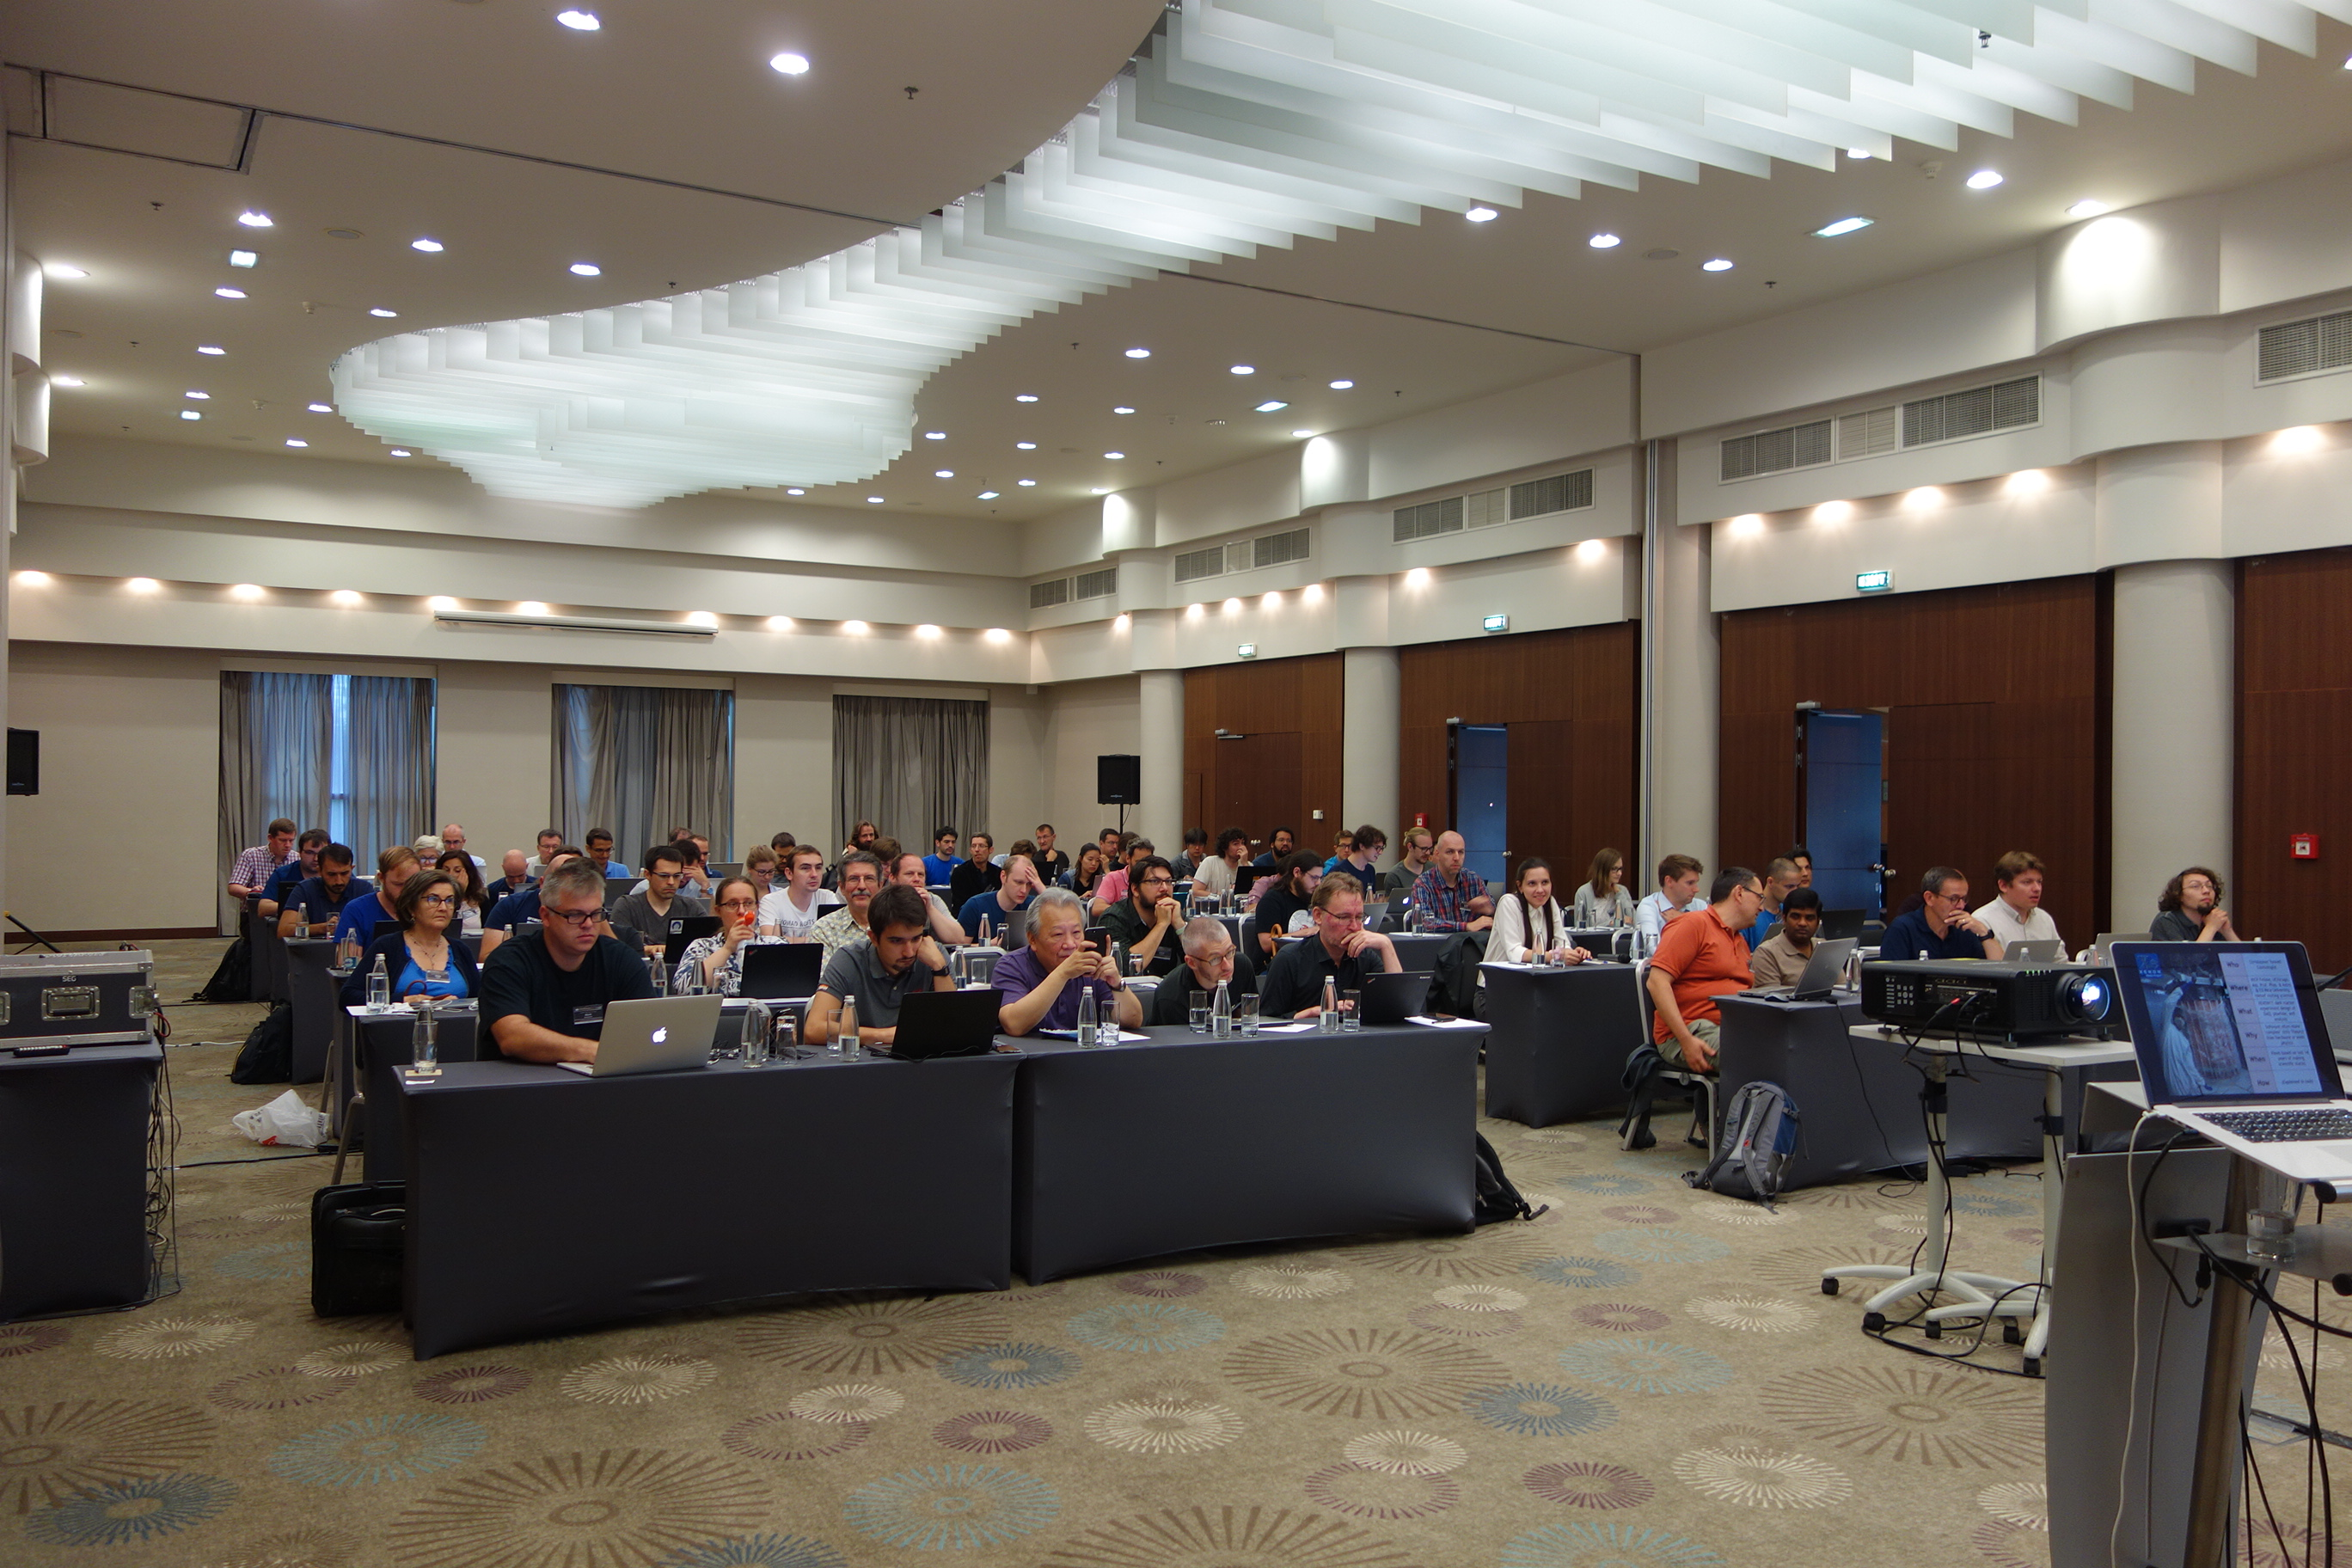
\includegraphics[width=\linewidth]{PLOTS/pyhep-2018-photo.jpg}

\column{0.5\linewidth}
\includegraphics[width=\linewidth]{PLOTS/pyhep-2021-photo.png}

\end{columns}

\vspace{0.1 cm}
\begin{columns}
\column{0.5\linewidth}
\mbox{ } \hfill 2018 \hfill \mbox{ }

\column{0.5\linewidth}
\mbox{ } \hfill 2021 \hfill \mbox{ }

\end{columns}
\end{frame}

\begin{frame}{Can you guess what happened?}
\vspace{0.5 cm}

\begin{columns}
\column{1.07\linewidth}
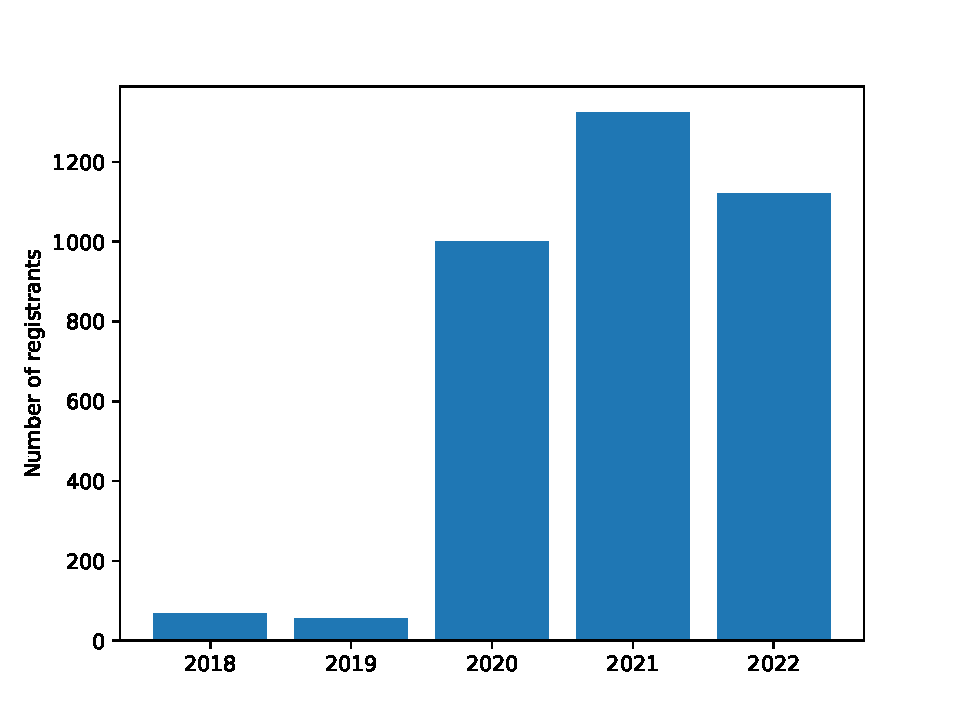
\includegraphics[height=5 cm]{PLOTS/pyhep-registration.pdf}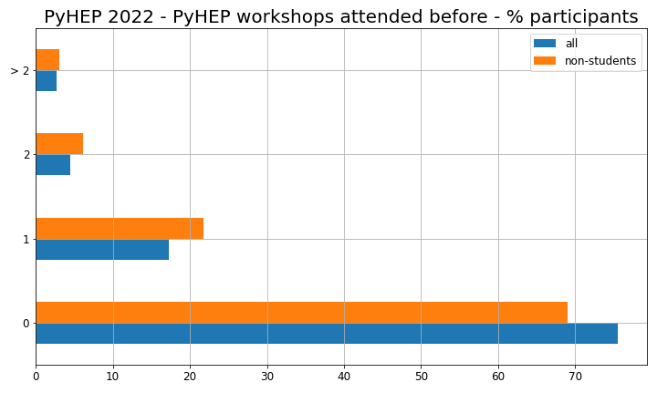
\includegraphics[height=5 cm]{PLOTS/pyhep-2022-attended-before.pdf}
\end{columns}

\vspace{1 cm}
\uncover<2->{By going virtual, we discovered a cohort of newcomers who can't/wouldn't travel.}
\end{frame}

\begin{frame}{About 20--40\% of the 1000 registrants attend/run the notebooks}
\vspace{0.5 cm}

\begin{columns}
\column{1.1\linewidth}
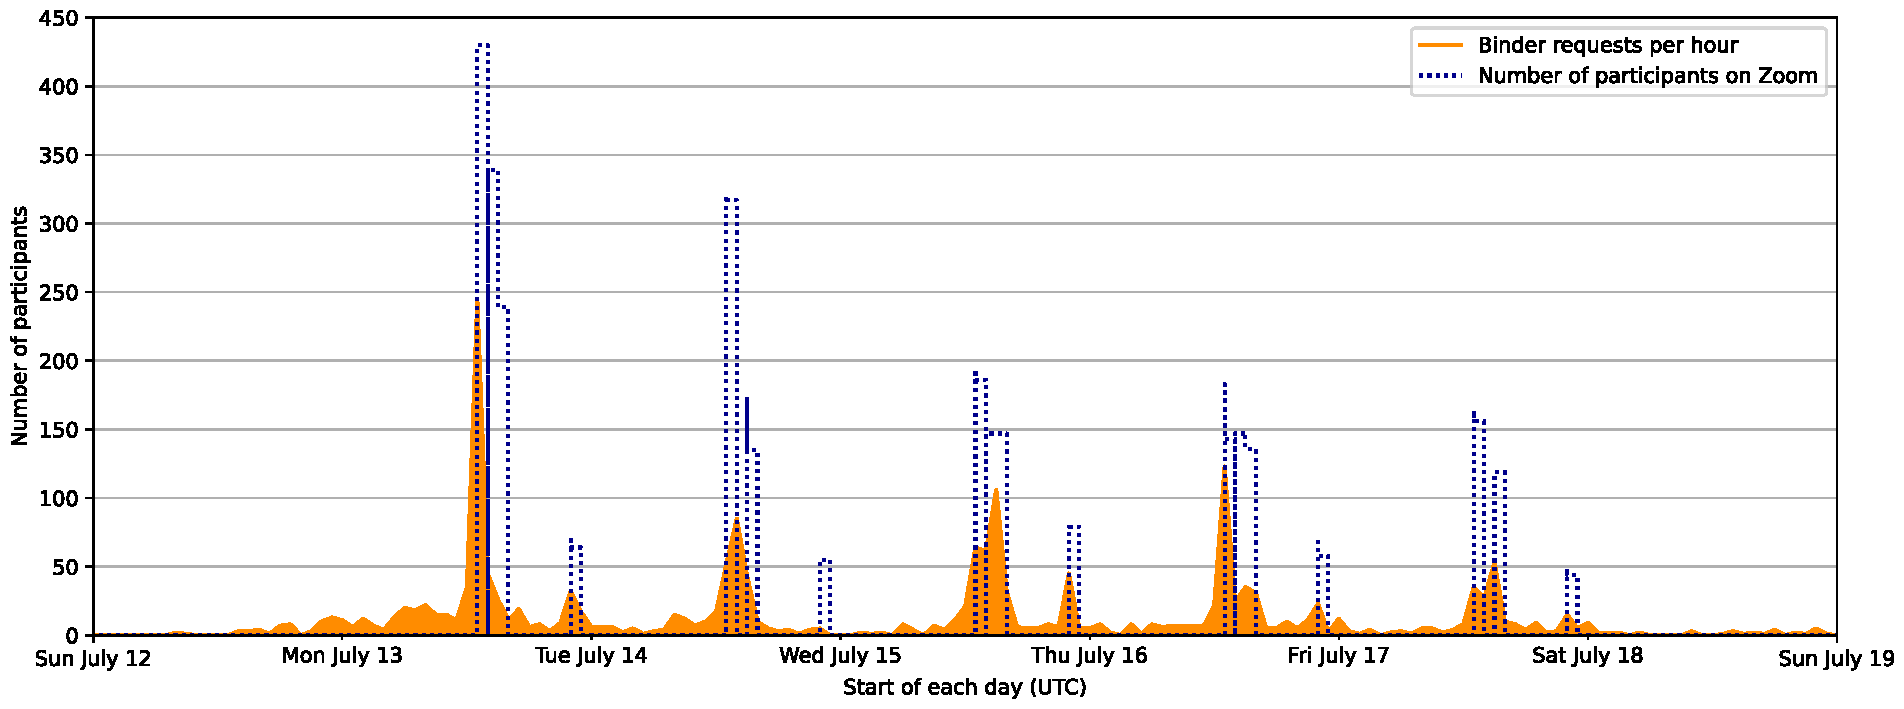
\includegraphics[width=\linewidth]{PLOTS/binder-launches-zoom-attendance.pdf}
\end{columns}
\end{frame}

\begin{frame}{In addition, there's the HSF/IRIS-HEP software training}
\vspace{1.25 cm}

\mbox{\hspace{-0.75 cm}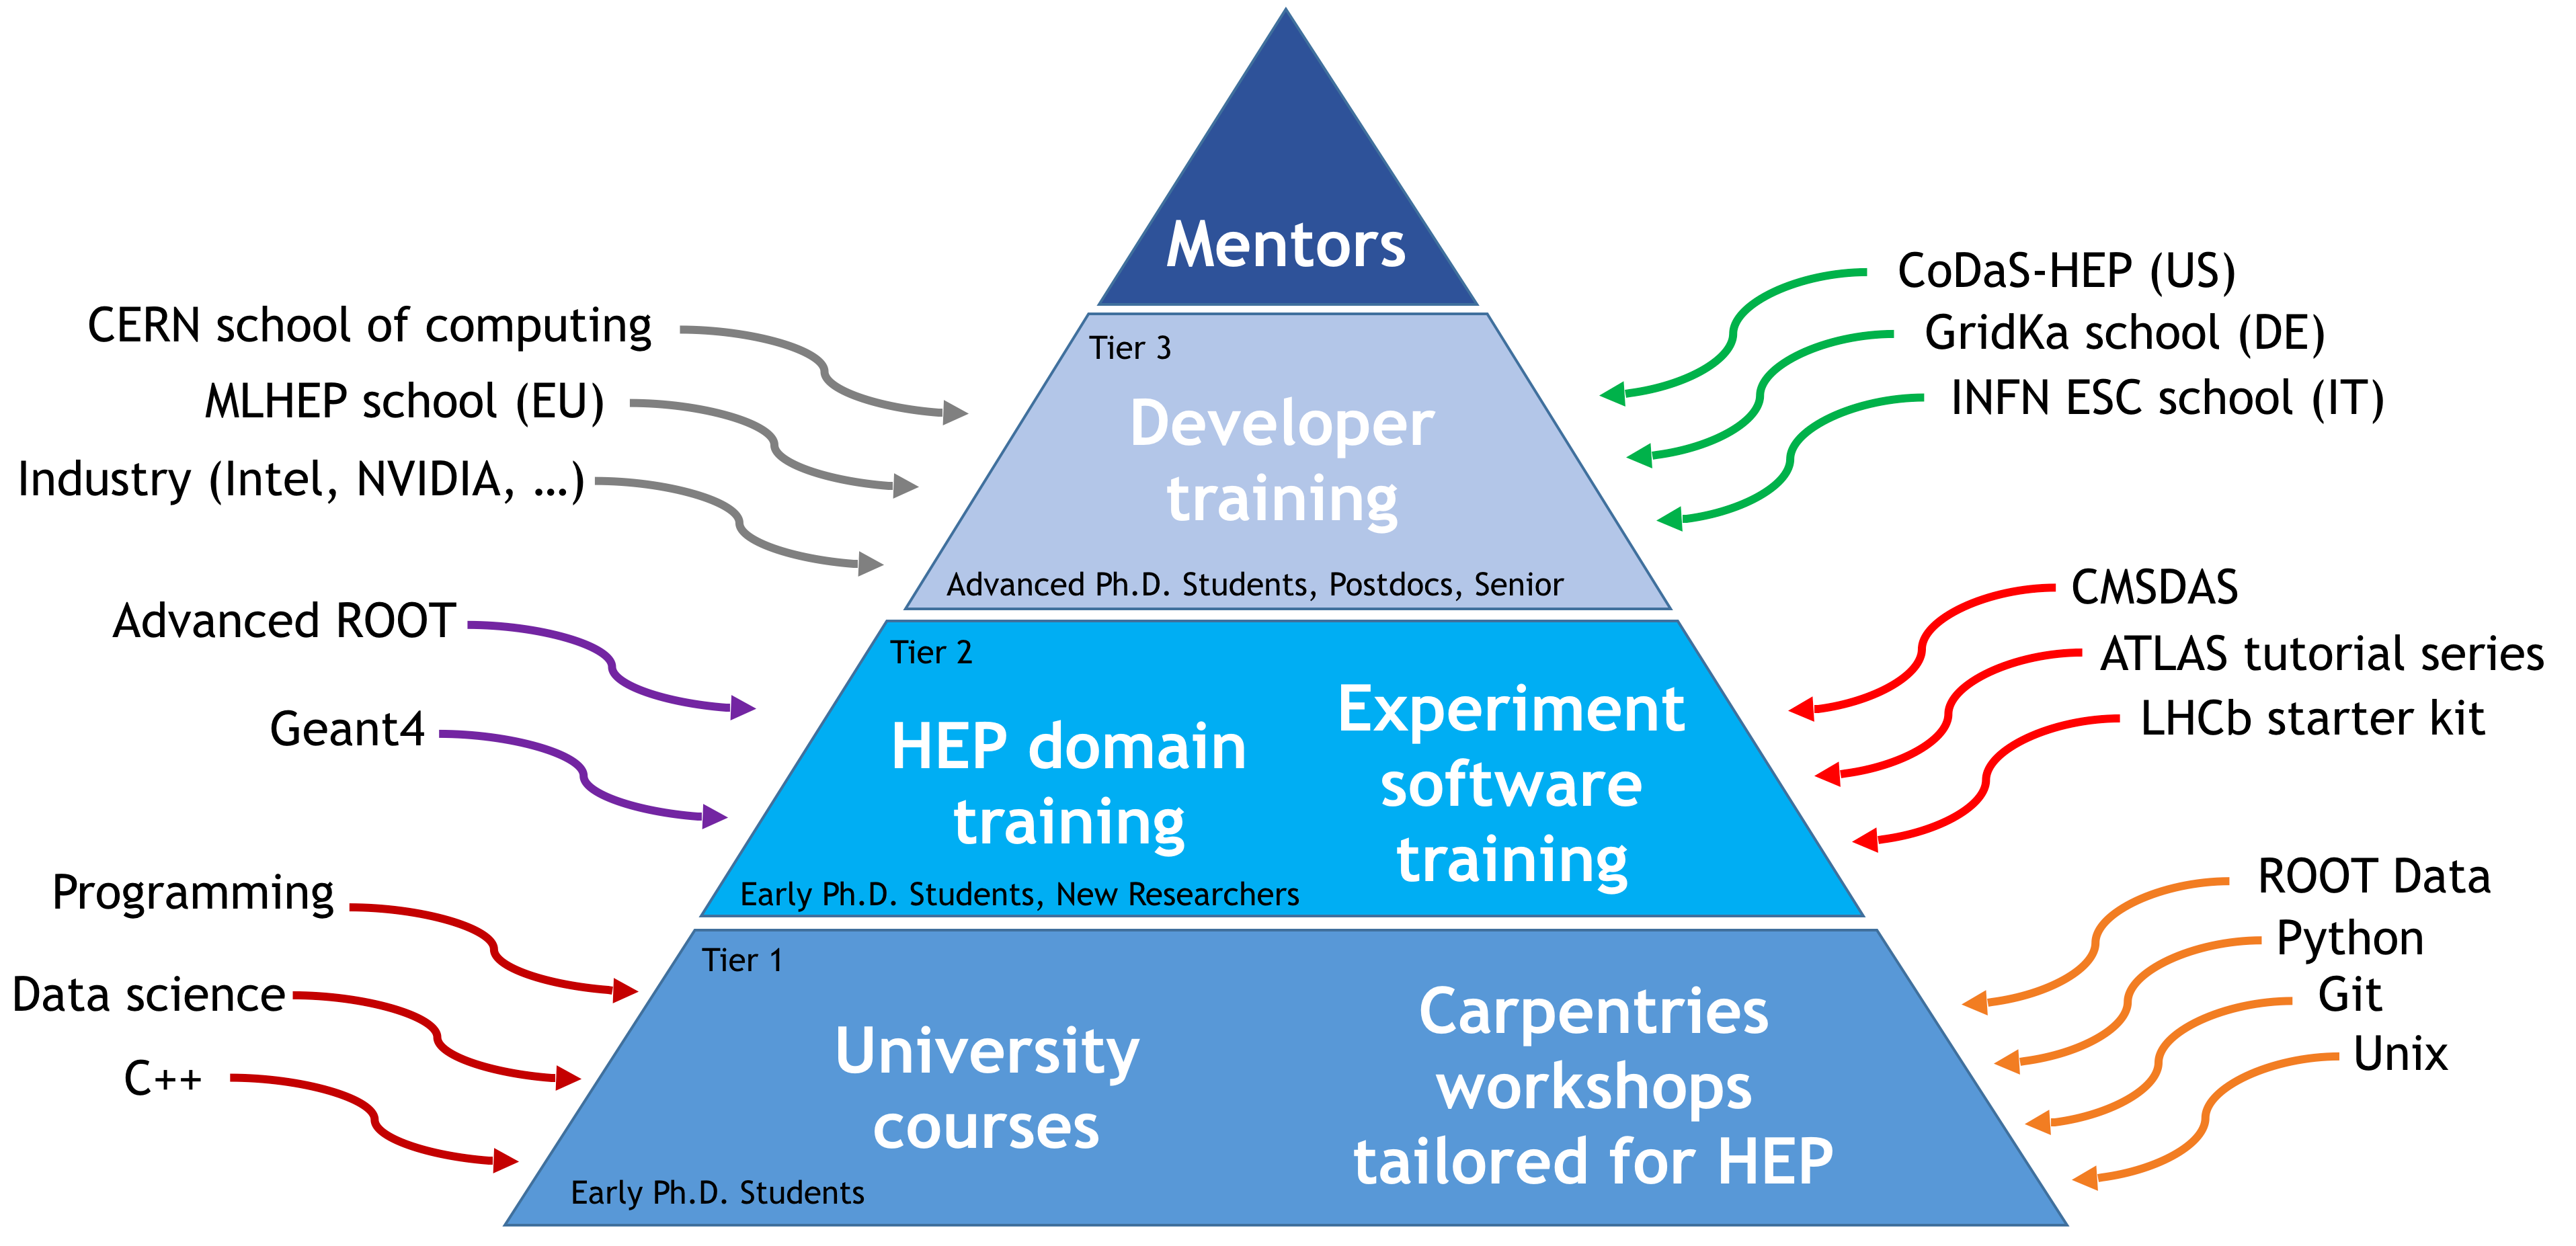
\includegraphics[width=\linewidth]{PLOTS/Training-Pyramid.png}}

\vspace{-7.75 cm}
\hfill \mbox{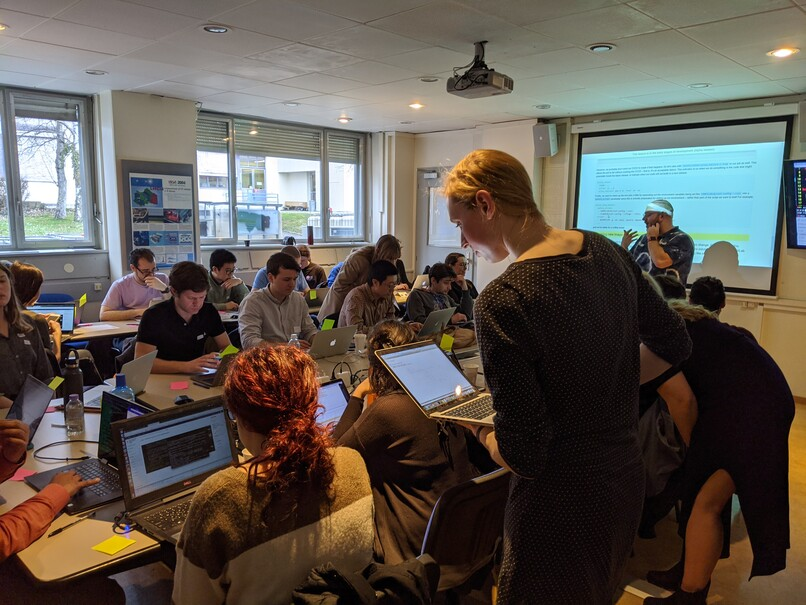
\includegraphics[width=4 cm]{PLOTS/instructor_mentor_small.jpg}\hspace{-1 cm}}
\vspace{7.75 cm}
\end{frame}

\begin{frame}{Where are we as a community?}
\Large

Well, we're using Python for data analysis a lot more.

\vspace{1 cm}
But more importantly, we're sharing (both ways) with the broader scientific community and making everything work together.
\end{frame}

\begin{frame}{My slide from Future Trends in Nuclear Physics Computing 2017}
\vspace{0.5 cm}
{\small\textcolor{blue}{\href{https://indico.jlab.org/event/213/contributions/2154/}{Lowering Boundaries between \\ Data Analysis Ecosystems}}, May 3, 2017}

\vspace{-1 cm}
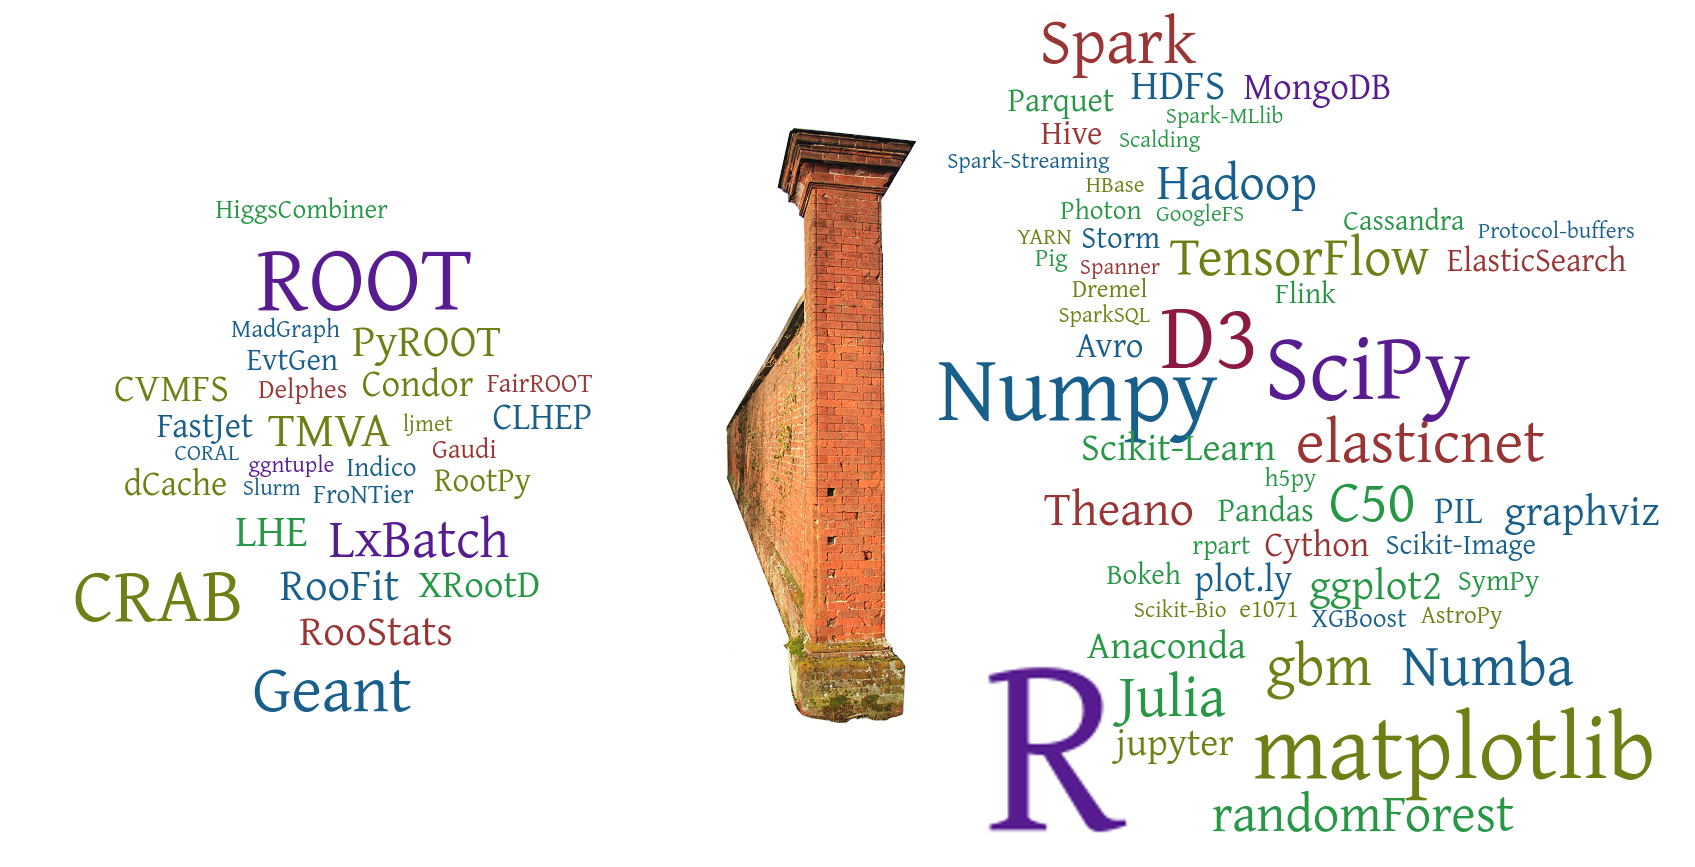
\includegraphics[width=\linewidth]{PLOTS/separation.png}

\vspace{-0.5 cm}
Evaluating this today, I'd say {\bf the wall is down.}
\end{frame}


\end{document}
